% CapSorter Research Paper — Structured & Composed via the PaperOrchestra Multi-Agent Pipeline
% Two-column conference manuscript format (CVPR/IEEE style)
\documentclass[10pt,twocolumn,letterpaper]{article}

\usepackage[pagenumbers]{cvpr}
%
% --- inline annotations
%
\newcommand{\red}[1]{{\color{red}#1}}
\newcommand{\todo}[1]{{\color{red}#1}}
\newcommand{\TODO}[1]{\textbf{\color{red}[TODO: #1]}}
% --- disable by uncommenting  
% \renewcommand{\TODO}[1]{}
% \renewcommand{\todo}[1]{#1}



\usepackage{iftex}
\ifXeTeX
  \usepackage{fontspec}
  \setmainfont{texgyretermes-regular.otf}[
    BoldFont = texgyretermes-bold.otf,
    ItalicFont = texgyretermes-italic.otf,
    BoldItalicFont = texgyretermes-bolditalic.otf,
  ]
  \setmonofont[Scale=0.80]{lmmono10-regular.otf}
\else
  \usepackage[T1]{fontenc}
\fi

\usepackage{multirow}
\usepackage{array}
\usepackage{algorithm}
\usepackage{algorithmic}
\usepackage{microtype}

\definecolor{cvprblue}{rgb}{0.21,0.49,0.74}
\usepackage[pagebackref,breaklinks,colorlinks,allcolors=cvprblue]{hyperref}
\usepackage[capitalize]{cleveref}

\title{CapSorter: An Air-Gapped Dual-Controller Vision-Guided Cartesian Pick-and-Place Architecture with Pipelined Bin-Side Re-Imaging and Fail-Safe Recovery}

\author{
Neil Shettigar$^{1}$\thanks{Lead embedded architecture, vision algorithms, firmware, and documentation. Interactive engineering portal and source repository: \url{https://capsorter.vercel.app} and \url{https://github.com/Neilboss/CapSorter}.} \qquad
Kahan$^{1}$ \qquad
Shourya$^{1}$\\[4pt]
$^{1}$CapSorter Autonomous Robotics Engineering Group
}

\begin{document}
\maketitle

% =========================================================================
% ABSTRACT
% =========================================================================
\begin{abstract}
Automated sorting of post-consumer plastic beverage bottle caps ($\varnothing 28\text{--}32\text{ mm}$) across unconstrained flat surfaces remains challenging for low-cost desktop robotic systems. Existing hobbyist and educational sorters frequently tether perception to cloud servers or external laptops, execute brittle open-loop batch plans that fail when parallel jaws displace adjacent caps on unpocketed trays, neglect wide-angle lens distortion and finite object-height parallax, and omit deterministic fail-safe recovery under serial communication loss. We present \textbf{CapSorter}, a completely air-gapped, dual-controller vision-guided Cartesian pick-and-place architecture operating across a continuous $300\times 300\text{ mm}$ open plywood workspace with four external color-sorting bins. CapSorter strictly decouples high-level computer vision and grasp planning from hard-real-time stepper actuation and hardware safety across two protocol-compatible front-ends sharing an identical Arduino Mega 2560 motion controller and CRC-16/CCITT-FALSE binary UART protocol: \textbf{Version~1 (V1)}, pairing an ESP32-CAM (OV2640) with a bare-metal $600\text{ MHz}$ Teensy~4.1 Cortex-M7 in $359.0\text{ KiB}$ of static \texttt{DMAMEM}; and \textbf{Version~2 (V2)}, consolidating vision and a native $480\times 320$ SPI touchscreen HUD (auto-detecting 16-bpp RGB565 / 32-bpp XRGB8888 framebuffers) onto an offline Raspberry Pi Zero~2~W (OS Lite) with a $160^\circ$ Sony IMX219 MIPI CSI-2 camera bridged to Mega \texttt{Serial1} via Micro-USB OTG and a level-shifted CH9102/CP2102 USB-to-TTL converter under fail-closed dual-model calibration. To solve open-plate neighbor disturbances without sacrificing throughput, we introduce \emph{closed-loop pipelined bin-side re-imaging} (\texttt{CMD\_SCAN\_WINDOW\_OPEN}), overlapping fresh board capture inside the $800\text{ ms}$ bin-drop sequence, paired with radial cap-height parallax compensation, distance-transform splitting of touching same-color caps, X-axis jaw-footprint clearance-first peeling, bridge-occlusion masking with mandatory clear-FOV verification parking, and a deterministic comms-loss finish-and-park state machine. Through a 28-test automated verification and end-to-end SIL suite (plus 8 staged bench bring-up utilities), synthetic-optics calibration benchmarks, and Monte Carlo software-in-the-loop (SIL) ablations across $N=50$ cluttered boards ($600$ caps), we demonstrate $24.4\times$ fisheye error reduction ($7.15\to 0.29\text{ mm}$), $62.5\times\text{--}116.8\times$ radial parallax reduction ($\le 0.43\text{ mm}$ residual), $100.0\%$ F1 cluster splitting on V2, and $100.0\%$ sorting completion versus $67.5\%$ open-loop while cutting V2 cycle time by $32.2\%$ ($9.48\text{ s/cap}$) over home-park re-imaging. Physical bench validation (operationalized via an 8-stage hardware bring-up procedure) remains an explicitly documented pre-deployment gate.
\end{abstract}

% =========================================================================
% SECTION 1: INTRODUCTION
% =========================================================================
\section{Introduction}
\label{sec:intro}

Global plastic production has surpassed $8.3\text{ billion}$ metric tons, with less than $10\%$ successfully recycled due largely to material contamination and mixed-polymer waste streams \cite{geyer2017production}. Beverage bottle caps—typically molded from high-density polyethylene (HDPE) or polypropylene (PP) with outer diameters of $\varnothing 28\text{--}32\text{ mm}$ and heights of $h_{\mathrm{cap}}\approx 13\text{ mm}$—represent a high-volume, color-differentiated packaging stream whose automated separation directly improves secondary recyclate purity \cite{gundupalli2017review,wilts2021artificial}. While industrial material recovery facilities deploy high-speed robotic delta sorters backed by hyperspectral arrays and GPU workstations \cite{lukka2014zenrobotics,koskinopoulou2021robotic,kiyokawa2023challenges}, translating reliable vision-guided sorting into compact, affordable, air-gapped tabletop robotics exposes four coupled engineering failure modes:

\begin{enumerate}
  \item \textbf{Host/Cloud Dependency and Real-Time Step Jitter.} Many low-cost sorters either offload perception to cloud APIs and ROS workstations \cite{hossen2025wastesortbot} or attempt to run vision and motor pulse generation concurrently on a single general-purpose operating system \cite{pereira2014lowcost}. Cloud dependence breaks offline reliability, while non-real-time OS scheduling introduces stepper pulse jitter and unpredictable fault-stop latencies.
  \item \textbf{Open-Plate Neighbor Disturbance (``Bump Failure'').} When caps rest freely on an unpocketed flat plate rather than in machined grid cavities, lowering a parallel two-finger gripper onto one cap routinely grazes adjacent caps and nudges them by $10\text{--}35\text{ mm}$. Open-loop batch planners that capture a single image at session start subsequently execute blind grasps at stale coordinates, driving steep sorting failure rates in clutter.
  \item \textbf{Optical Distortion, Finite-Height Parallax, and Touching Silhouettes.} Compact desktop frames ($500\text{ mm}$ height) force overhead cameras close to the workspace ($H_{\mathrm{cam}}\approx 200\text{--}400\text{ mm}$), requiring wide-angle lenses (e.g., $160^\circ$ fisheye) that exhibit $>20\text{ mm}$ peripheral barrel distortion if unrectified \cite{kannala2006generic}. Even after exact planar homography at $Z=0$ \cite{hartley2004multiple}, the cap top sits $h_{\mathrm{cap}}\approx 13\text{ mm}$ above the board, creating outward radial parallax errors exceeding the $\pm 3.0\text{ mm}$ jaw half-clearance near corners. Simultaneously, naive contour centroiding merges touching same-color caps into invalid midpoints between objects.
  \item \textbf{Inadequate Electrical Safety and Link-Loss Recovery.} Educational robotic builds rarely enforce fail-closed camera calibration guards, bidirectional $3.3\text{ V}\leftrightarrow 5.0\text{ V}$ serial protection, hardwired dual-pole emergency stops \cite{iso13850}, or deterministic behavior when inter-controller UART supervision drops mid-cycle.
\end{enumerate}

To address all four limitations simultaneously without external PCs, Wi-Fi, or cloud infrastructure, we introduce \textbf{CapSorter}, a $500\times 500\times 500\text{ mm}$ offline dual-controller Cartesian pick-and-place architecture. CapSorter isolates real-time stepper/servo timing and hardware safety on an Arduino Mega~2560 while exposing a unified, CRC-16/CCITT-FALSE protected binary UART interface supporting two complete vision architectures: \textbf{V1} (bare-metal ESP32-CAM + Teensy~4.1 Cortex-M7) and \textbf{V2} (consolidated Raspberry Pi Zero~2~W + $3.5\text{ in}$ SPI Touch LCD HUD + $160^\circ$ Sony IMX219 MIPI CSI-2 camera bridged via Micro-USB OTG CH9102/CP2102). Our principal contributions are:
\begin{itemize}
  \item \textbf{Dual-Architecture Air-Gapped Hardware Partitioning (\cref{sec:hardware}):} A comparative bare-metal MCU (V1) versus edge-Linux SBC (V2) architecture sharing one deterministic Mega~2560 motion/safety controller, a 3-branch common star-ground power distribution tree, bidirectional $3.3\text{ V}\leftrightarrow 5.0\text{ V}$ level shifting, polled Port~A normally-closed (NC) limit switches with pre-homing broken-wire verification, and a hardwired dual-pole latching E-stop.
  \item \textbf{Fail-Closed Vision, Radial Parallax Correction, and Touching-Cap Separation (\cref{sec:method}):} A metadata-enforced dual-model (Kannala--Brandt fisheye / pinhole) calibration pipeline, closed-form radial height parallax correction, and direct comparison between memory-bounded $L_1$ chessboard chamfer splitting (V1, $25.0\text{ KiB}$ $160\times 160$ ROI) and gap-preserving $L_2$ Euclidean peak splitting (V2).
  \item \textbf{Pipelined Bin-Side Re-Imaging with Clearance-First Peeling (\cref{sec:method}):} A closed-loop single-target protocol (\texttt{0x5B} / \texttt{0xA5}) that overlaps fresh overhead capture with the $800\text{ ms}$ bin-drop sequence, coupled with exact 2D circle--rectangle X-jaw collision avoidance, $\pm 35\text{ mm}$ Y-bridge occlusion masking, clear-FOV verification parking (\texttt{0xB5}), and 3-attempt missed-pick quarantine guaranteeing finite termination.
  \item \textbf{Deterministic Comms-Loss Finish-and-Park Policy (\cref{sec:method}):} Continuous $250\text{ ms}$ heartbeat supervision (interleaved even inside V1's $1.67\text{ s}$ UART2 frame stream) with a $1.2\text{ s}$ watchdog that completes only an actively dispatched cap, parks at $(0,0)$, de-energizes steppers, and latches fault state until explicit operator re-arm and re-homing.
  \item \textbf{Comprehensive SIL, Synthetic-Optics, and Staged Bring-Up Verification (\cref{sec:experiments}):} Reproducible evaluation across $28$ automated unit and end-to-end SIL tests (including non-zero tool-offset frame separation, mid-cap UART-cut finish-and-park-and-rearm, mid-session LCD pause, USB-TTL reconnect, and smoke tests of 8 staged hardware bring-up utilities), $64$-point optical calibration grids, $5$ touching-cluster geometries, $N=50$ Monte Carlo cluttered boards ($600$ caps), $11{,}664$ kinematic transitions, and $15{,}000$ CRC-16 fault injections, clearly delineating verified software behavior from the pending Stages~0--8 physical bench gate (\cref{sec:limitations}).
\end{itemize}

\begin{figure*}[t]
  \centering
  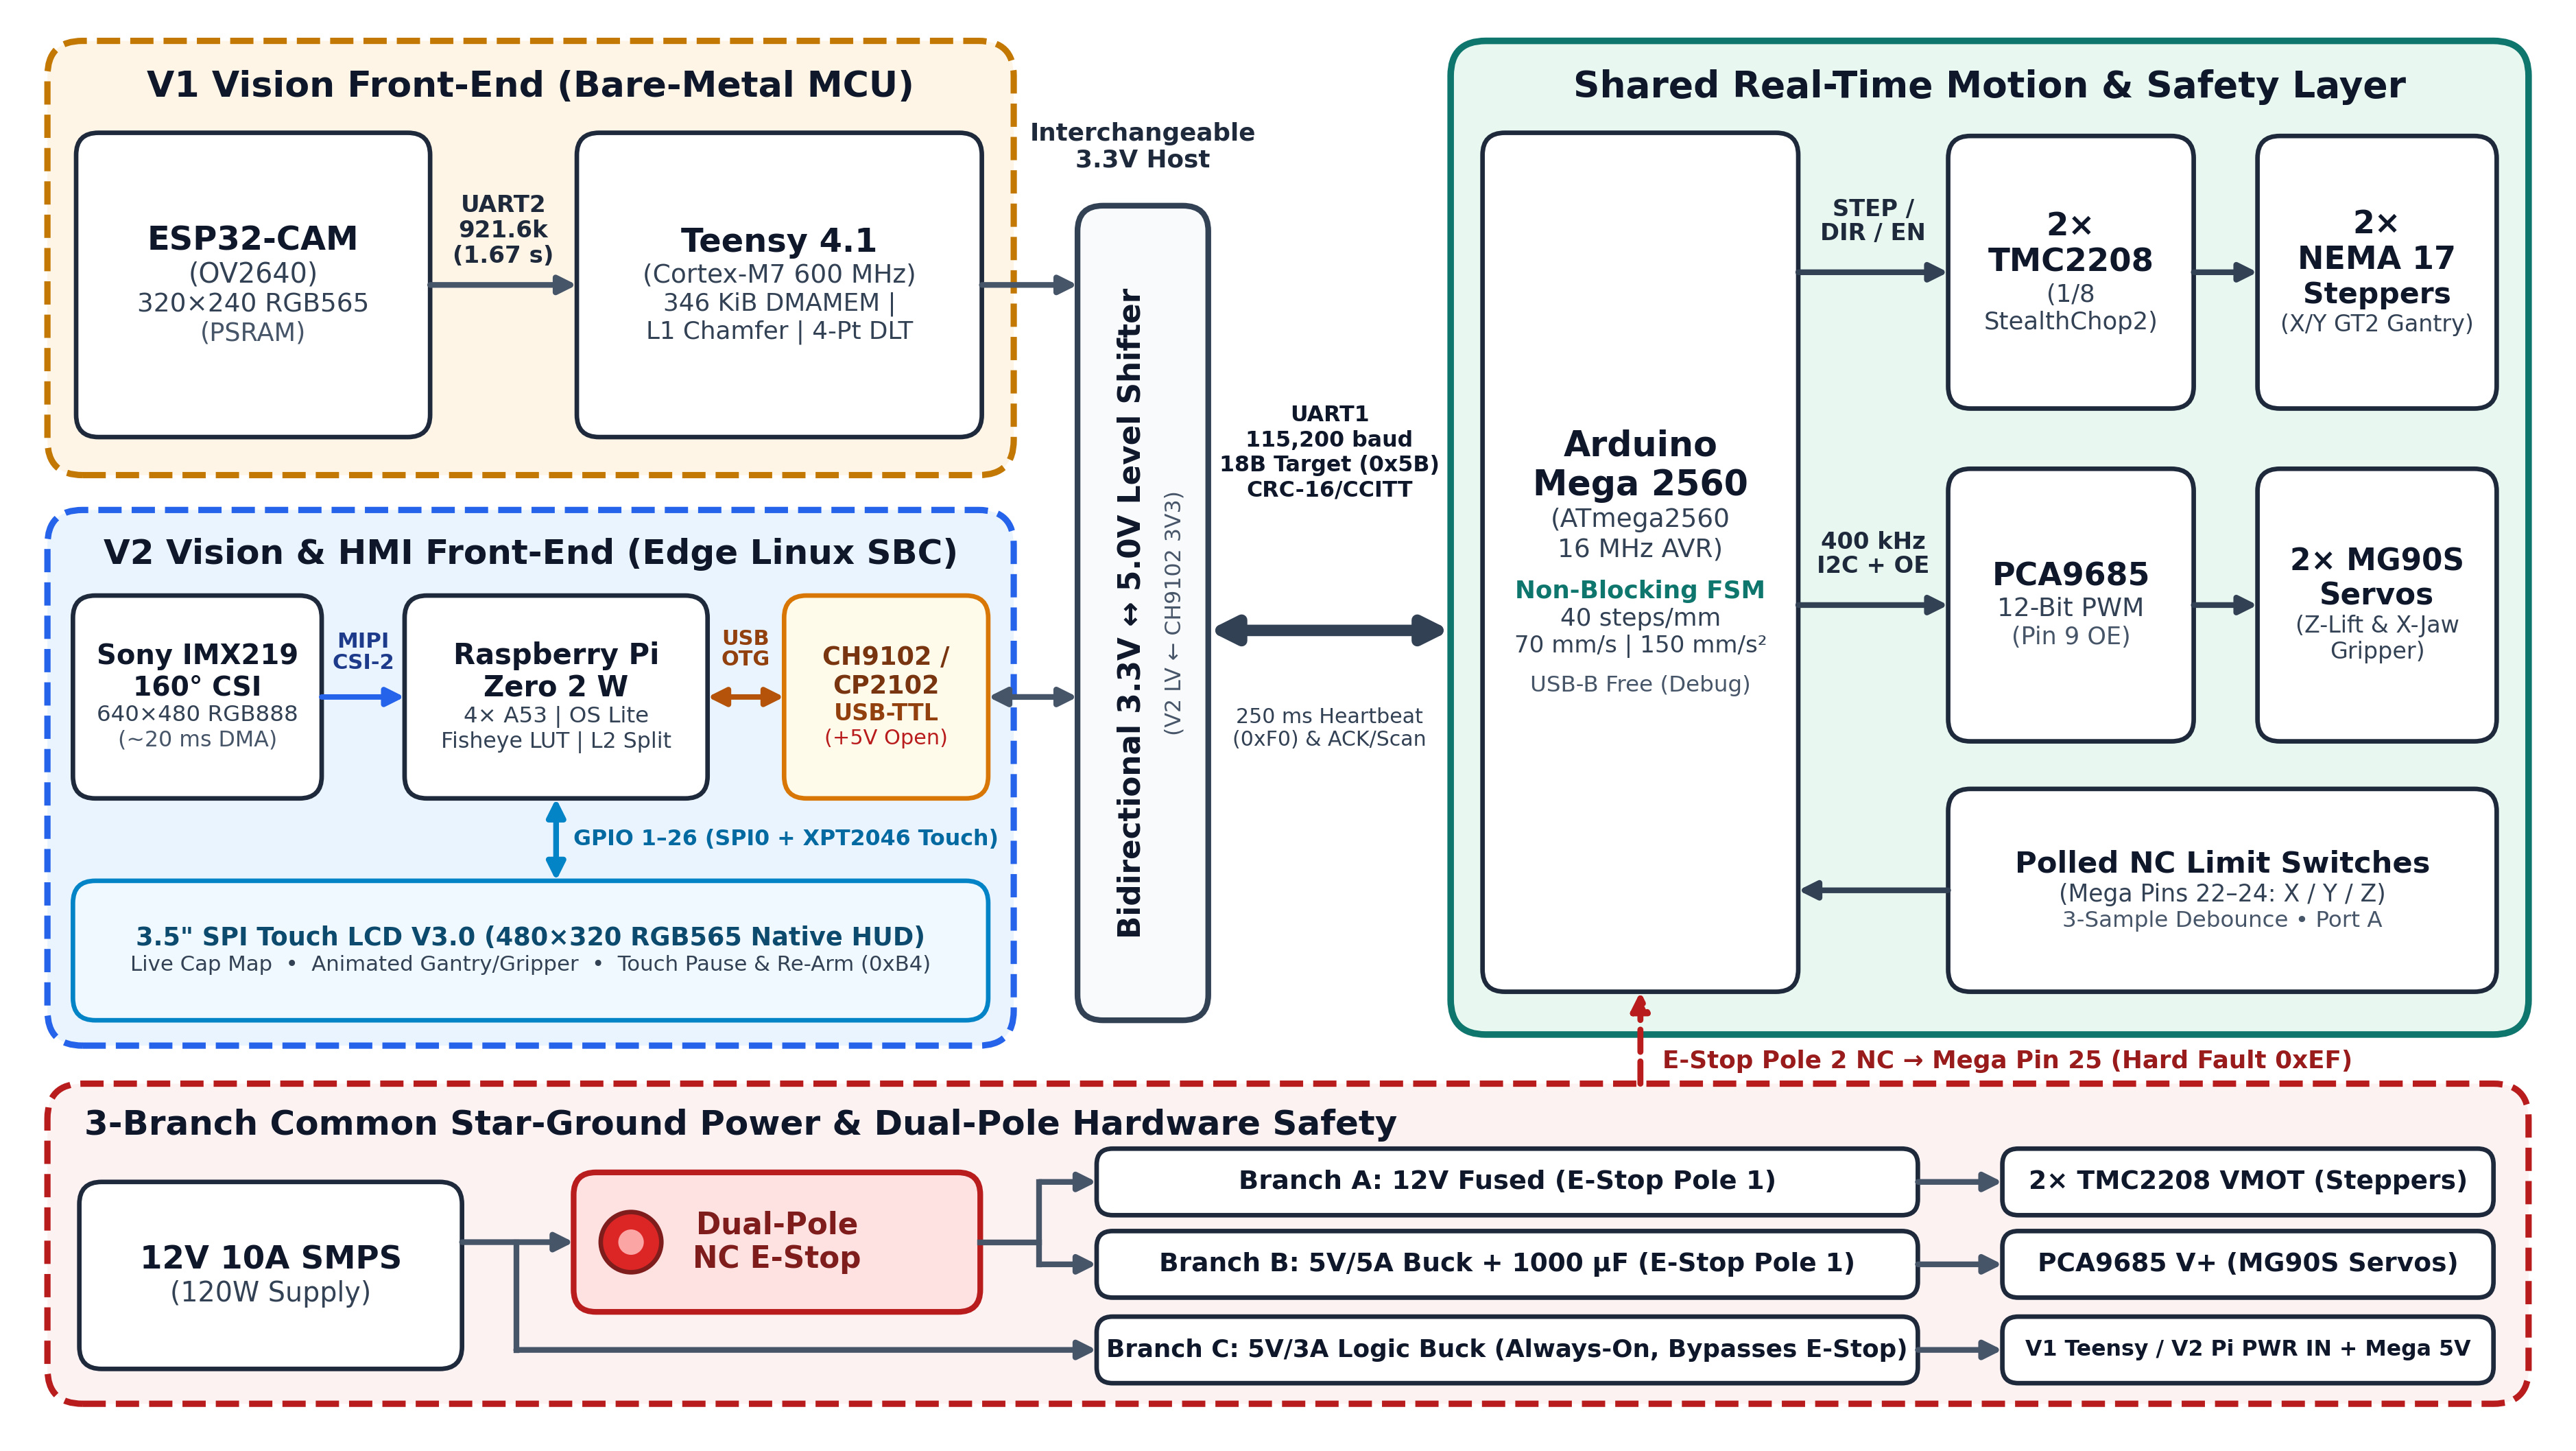
\includegraphics[width=\textwidth]{figures/fig_system_architecture.jpg}
  \caption{Dual-architecture offline hardware and safety partitioning of \textbf{CapSorter}. Two interchangeable $3.3\text{ V}$ vision front-ends—\textbf{V1} (ESP32-CAM OV2640 streaming QVGA RGB565 over $921.6\text{ kbps}$ UART2 to a bare-metal $600\text{ MHz}$ Teensy~4.1) and \textbf{V2} (8MP Sony IMX219 $160^\circ$ CSI camera feeding a quad-core Raspberry Pi Zero~2~W with a $3.5\text{ in}$ SPI Touch LCD on GPIO~1--26 and a Micro-USB OTG $\to$ CH9102/CP2102 USB-TTL bridge)—connect through a mandatory bidirectional $3.3\text{ V}\leftrightarrow 5.0\text{ V}$ level shifter to a shared real-time Arduino Mega~2560 motion and safety layer. A $12\text{ V}/10\text{ A}$ SMPS drives three separate regulated branches sharing a common star ground: Pole~1 of a dual-pole latching NC E-stop hard-cuts actuator Branches~A and~B, Branch~C bypasses the E-stop (feeding V2 Pi Zero~2~W via \texttt{PWR IN} Micro-USB) to preserve logic telemetry and SD integrity, and Pole~2 signals Mega Pin~25 to latch \texttt{STATE\_HARD\_FAULT} (\texttt{0xEF}).}
  \label{fig:architecture}
\end{figure*}

% =========================================================================
% SECTION 2: RELATED WORK
% =========================================================================
\section{Related Work}
\label{sec:related_work}

\subsection{Vision-Guided Automated Waste and Object Sorting}
Automated waste sorting has progressed rapidly from mechanical trommels and eddy-current separators toward vision-guided robotic manipulators \cite{gundupalli2017review,wilts2021artificial}. Industrial deployments such as the ZenRobotics Recycler \cite{lukka2014zenrobotics} and multi-sensor recyclable separation cells \cite{koskinopoulou2021robotic,kiyokawa2023challenges} achieve high throughput on conveyor streams using deep neural detectors and pneumatic or delta-arm actuators, but require multi-kilowatt infrastructure and workstation GPUs unsuitable for compact, low-cost settings. Conversely, accessible sorting prototypes built around Raspberry Pi and Arduino controllers \cite{pereira2014lowcost} or ROS-cloud stacks such as WasteSortBot \cite{hossen2025wastesortbot} rely either on structured single-file feeding, cloud connectivity, or open-loop single-pass perception. CapSorter occupies the underserved middle ground: a self-contained, air-gapped desktop Cartesian gantry capable of sorting dense, arbitrary multi-cap layouts on an open flat surface with industrial-grade protocol integrity and hardware safety.

\subsection{Calibration, Parallax, and Touching-Blob Separation}
Metric 2D manipulation from monocular overhead imaging builds on planar checkerboard intrinsic calibration \cite{zhang2000flexible}, projective 4-point Direct Linear Transform (DLT) homography \cite{hartley2004multiple}, and wide-angle equidistant lens modeling \cite{kannala2006generic}, widely implemented via OpenCV \cite{bradski2000opencv}. In compact enclosures, wide-angle fisheye lenses preserve full workspace coverage at low mounting heights ($H_{\mathrm{cam}} \le 300\text{ mm}$) but introduce severe peripheral distortion unless explicitly rectified \cite{kannala2006generic}; moreover, projecting elevated object tops onto a $Z=0$ calibrated plane introduces systematic radial parallax error that scales inversely with $H_{\mathrm{cam}}$. For color segmentation under controlled lighting, perceptual Hue-Saturation-Value (HSV) transforms \cite{smith1978color} coupled with topological border following \cite{suzuki1985topological} provide robust, compute-light localization on embedded targets compared to microcontroller deep-learning stacks \cite{lin2020mcunet}. However, binary contour extraction merges touching same-color parts. Classical watershed immersion \cite{vincent1991watersheds} and distance transforms—including Borgefors' memory-efficient two-pass chamfer approximations \cite{borgefors1986distance} and exact linear-time Euclidean transforms \cite{felzenszwalb2012distance}—resolve touching circular geometries. CapSorter directly benchmarks a $25.0\text{ KiB}$ bare-metal $L_1$ chamfer splitter (V1) against an interior-gap-preserving $L_2$ Euclidean peak splitter (V2) on identical touching-cap benchmarks.

\subsection{Cluttered Grasp Planning and Safety-Critical Control}
Grasping in dense clutter has been extensively studied through analytical and learned grasp-quality policies such as Dex-Net~4.0 \cite{mahler2019learning}, multi-affordance pick-and-place \cite{zeng2018robotic}, pushing-grasping synergies \cite{zeng2018learning}, and multi-step mechanical search under occlusion \cite{danielczuk2019mechanical}. While deep affordance policies excel on diverse 3D objects using RGB-D sensors and GPUs, planar sorting of uniform cylindrical caps with a fixed-orientation parallel gripper admits an exact geometric clearance formulation: modeling descending jaw envelopes as axis-aligned rectangles allows deterministic $O(N^2)$ outside-in cluster peeling on a microcontroller. Furthermore, classical look-and-move visual servoing \cite{chaumette2006visual} typically incurs a stop-and-look latency penalty when re-imaging after each pick. CapSorter eliminates this penalty on V2 by pipelining overhead re-imaging during bin-side drop dwells. Finally, reliable embedded robotics requires strict separation between best-effort perception and deterministic actuation, CRC polynomials selected for maximum Hamming distance over short payloads \cite{koopman2004cyclic}, and hardwired latching emergency stops adhering to ISO~13850 design principles \cite{iso13850}.

% =========================================================================
% SECTION 3: HARDWARE, KINEMATICS & SAFETY ARCHITECTURE
% =========================================================================
\section{System Hardware, Kinematics, and Electrical Safety}
\label{sec:hardware}

\subsection{Dual-Controller Partitioning: V1 vs. V2}
\Cref{fig:architecture} illustrates CapSorter's architectural separation across two complete, interchangeable vision front-ends coupled to one shared real-time motion controller. Detailed specifications are contrasted in \cref{tab:hardware_comparison}.

\begin{table*}[t]
  \centering
  \footnotesize
  \setlength{\tabcolsep}{4.5pt}
  \begin{tabular}{@{}p{3.1cm}p{6.65cm}p{6.65cm}@{}}
    \toprule
    \textbf{Subsystem / Parameter} & \textbf{Version 1 (Bare-Metal Dual-MCU)} & \textbf{Version 2 (Consolidated Edge SBC)} \\
    \midrule
    Primary Vision Processor & Teensy~4.1 (NXP i.MX RT1062, $600\text{ MHz}$ M7, $1\text{ MB}$ SRAM) & Raspberry Pi Zero~2~W ($4\times 1.0\text{ GHz}$ A53, $512\text{ MB}$) + $3.5\text{ in}$ SPI Touch LCD \\
    Camera Sensor \& Link & ESP32-CAM OV2640, $320\times 240$ RGB565 via UART2 ($921.6\text{k}$) & Sony IMX219 $160^\circ$ CSI (2-lane DMA; USB cam needs hub) ($640\times 480$) \\
    Capture + Vision Latency & $\sim 1.67\text{ s}$ UART2 stream $+ \sim 40\text{ ms}$ C++ ($\approx 1.71\text{ s}$) & $\sim 20\text{ ms}$ MIPI CSI-2 DMA $+ \sim 25\text{ ms}$ OpenCV ($\approx 45\text{ ms}$) \\
    Lens Calibration Model & 4-pt DLT planar homography (\texttt{V1\_CALIBRATION\_VERIFIED}) & Fail-closed \texttt{.npz}: Kannala--Brandt fisheye or pinhole + $\mathbf{H}$ \\
    Cluster Splitting Method & Two-pass $3\times 3$ chessboard chamfer ($160\times 160$ ROI, $25.0\text{ KiB}$) & Gap-preserving $L_2$ Euclidean distance transform + Gaussian peaks \\
    Memory Management & $375.0\text{ KiB}$ static \texttt{DMAMEM} ($36.6\%$ SRAM, zero \texttt{malloc}) & Precomputed \texttt{CV\_16SC2} LUTs on offline 64-bit Linux \\
    \midrule
    \multicolumn{3}{@{}l}{\textbf{Shared Motion, Actuation, Protocol \& Safety Layer (Identical Across V1 and V2)}} \\
    \midrule
    Motion Controller & \multicolumn{2}{@{}p{13.5cm}@{}}{Arduino Mega~2560 Rev3 ($16\text{ MHz}$ ATmega2560), non-blocking \texttt{AccelStepper} FSM, $400\text{ kHz}$ I2C + $3\text{ ms}$ \texttt{Wire} timeout} \\
    XY Gantry Actuation & \multicolumn{2}{@{}p{13.5cm}@{}}{$2\times$ NEMA~17 ($1.3\text{ A}$, $4.2\text{ kg}\cdot\text{cm}$), $2\times$ TMC2208 ($1/8$ StealthChop2), 20T GT2 ($40.0\text{ steps/mm}$, $70\text{ mm/s}$, $150\text{ mm/s}^2$)} \\
    Z-Lift \& Gripper & \multicolumn{2}{@{}p{13.5cm}@{}}{PCA9685 12-bit $50\text{ Hz}$ PWM (\texttt{0x40}, \texttt{OE=Pin~9}) driving $2\times$ MG90S ($40\text{ mm}$ crank-slider Z; $36/26\text{ mm}$ X-jaws)} \\
    Inter-Controller Link & \multicolumn{2}{@{}p{13.5cm}@{}}{V1 GPIO / V2 Micro-USB OTG $\to$ CH9102/CP2102 $\leftrightarrow$ $3.3\leftrightarrow 5\text{ V}$ Shifter $\leftrightarrow$ Mega UART1 ($115.2\text{k}$, 18B \texttt{0x5B} CRC-16, $250\text{ ms}$ ping)} \\
    Power \& Safety Hardware & \multicolumn{2}{@{}p{13.5cm}@{}}{$12\text{ V}/10\text{ A}$ SMPS $\to$ 3 regulated branches (common star GND); dual-pole NC E-stop (Pin~25); polled NC limits (Pins~22--24)} \\
    \bottomrule
  \end{tabular}
  \caption{Comprehensive hardware and algorithmic comparison between CapSorter V1 (bare-metal dual-MCU) and V2 (consolidated edge SBC), highlighting the strictly shared real-time motion, wire protocol, and electrical safety layer.}
  \label{tab:hardware_comparison}
\end{table*}

\paragraph{Version~1 (Bare-Metal MCU Stack).}
In V1, an AI-Thinker ESP32-CAM executes pure frame acquisition with zero Wi-Fi/Bluetooth stack overhead. On boot, the firmware verifies external PSRAM availability (\texttt{psramFound()}), zero-initializes \texttt{camera\_config\_t} to prevent uninitialized driver struct fields, allocates double-buffered QVGA ($320\times 240$) RGB565 framebuffers ($153{,}600\text{ B}$ each) in PSRAM with \texttt{CAMERA\_GRAB\_LATEST}, allows $800\text{ ms}$ of automatic white-balance/exposure/gain convergence under the diffused LED light plate, flushes two warm-up frames, and locks AWB/AEC/AGC so differently colored caps cannot shift scene hue balance. Upon receiving \texttt{CMD\_CAPTURE\_FRAME} (\texttt{0xAA}) over UART2 ($921{,}600\text{ baud}$), the ESP32-CAM explicitly discards one buffered stale frame before capturing and streaming a framed payload in $4\text{ KiB}$ chunks interleaved with \texttt{yield()} for FreeRTOS watchdog safety: 2-byte sync \texttt{[0x55, 0xAA]}, 32-bit big-endian length, $153{,}600\text{ B}$ RGB565 data, and a 2-byte CRC-16/CCITT-FALSE trailer.

The Teensy~4.1 ($600\text{ MHz}$ ARM Cortex-M7, $1024\text{ KiB}$ SRAM) allocates all working buffers statically in \texttt{DMAMEM} (RAM2) with zero dynamic heap allocation: \texttt{imageBuffer} ($153{,}600\text{ B}$), \texttt{rawMask} ($76{,}800\text{ B}$), \texttt{colorMask} ($76{,}800\text{ B}$), circular \texttt{bfsQueue} ($8{,}192\times 4 = 32{,}768\text{ B}$, with explicit overflow rejection so truncated components never corrupt centroids), UART2 DMA receive ring buffer \texttt{serial2RxBuf} ($16{,}384\text{ B}$ to prevent drops at $921.6\text{ kbps}$), chamfer ROI \texttt{splitDistMap} ($160\times 160 = 25{,}600\text{ B}$, accommodating wide 4--5 cap same-color clusters), and retry/target metadata ($100$-slot \texttt{retryZones} + \texttt{detectedCaps}, $\sim 2{,}048\text{ B}$), totaling $384{,}000\text{ B}$ ($375.0\text{ KiB}$, or $36.6\%$ of total SRAM; \cref{fig:safety_fsm}c). Crucially, because streaming $153{,}600\text{ B}$ at $921{,}600\text{ baud}$ requires $\sim 1.67\text{ s}$—longer than the Mega's $1.2\text{ s}$ heartbeat timeout—Teensy's \texttt{receiveFrameWithHeartbeat()} actively services Mega \texttt{0xF0} pings every $250\text{ ms}$ and monitors fault opcodes mid-stream, returns \texttt{EXEC\_CAPTURE\_FAULT} (never \texttt{EXEC\_COMPLETE}) on capture/CRC failure, and accepts explicit operator \texttt{REARM} recovery over USB Serial (or an optional Pin~2 panel button) to emit \texttt{CMD\_REARM\_HOME}.

\paragraph{Version~2 (Consolidated Edge SBC + Local HMI Stack).}
V2 replaces both ESP32-CAM and Teensy~4.1 with a single offline Raspberry Pi Zero~2~W (quad-core $1.0\text{ GHz}$ Cortex-A53, $512\text{ MB}$ RAM, 64-bit Raspberry Pi OS Lite Bookworm) running Python~3.11 and OpenCV~4.x \cite{bradski2000opencv}. An 8MP Sony IMX219 $160^\circ$ wide-angle camera attaches over 2-lane MIPI CSI-2, configured via \texttt{Picamera2} with \texttt{raw=\{"size":(1640,1232)\}} to enforce full-sensor $2\times 2$ binning before ISP downscaling to $640\times 480$ \texttt{RGB888} (DRM byte-order $[B,G,R]$ matching OpenCV BGR) while preserving the full wide field of view. After an $800\text{ ms}$ warm-up, converged \texttt{ExposureTime}, \texttt{AnalogueGain}, and \texttt{ColourGains} are read from \texttt{capture\_metadata()} and latched explicitly alongside \texttt{AeEnable=False, AwbEnable=False} so \texttt{libcamera} cannot revert white balance to green-tinted unity gains. Direct CSI DMA slashes frame acquisition from $1.67\text{ s}$ (V1) to $\sim 20\text{ ms}$, yielding $\sim 45\text{ ms}$ total acquisition-plus-vision latency; a guarded background heartbeat thread (\texttt{\_GuardedHeartbeatSupervisor}) decouples $250\text{ ms}$ \texttt{0xF0} UART pings from transient capture/OpenCV jitter while enforcing a bounded $3.5\text{ s}$ vision liveness deadline so genuine deadlocks still trip Mega's safe halt. A $3.5\text{ in}$ SPI touchscreen LCD (V3.0, $480\times 320$, ILI9486/XPT2046) attaches directly to Pi GPIO pins~1--26 via Bookworm's native \texttt{dtoverlay=piscreen,drm} driver, running a lightweight $<20\text{ MB}$ native OpenCV framebuffer HUD (\texttt{lcd\_hud.py}, querying true \texttt{FBIOGET\_VSCREENINFO}/\texttt{FBIOGET\_FSCREENINFO} resolution, \texttt{line\_length} row stride, and RGB/BGR bitfields) without Desktop/Chromium bloat—animating detected caps and Mega-opcode-synchronized gantry motion while exposing tactile mid-session Pause (parking cleanly via \texttt{CMD\_FINISH\_SESSION}) and thread-safe \texttt{CMD\_REARM\_HOME} controls with configurable XPT2046 axis orientation. Because the 26-pin LCD header physically covers GPIO~14/15 UART0 and Pins~2/4/6, V2 connects to Mega \texttt{Serial1} through the Pi's inner Micro-USB OTG port via an Official OTG adapter and a WCH CH9102/CH343/CP2102 USB-to-TTL module (\texttt{/dev/capsorter\_mega} via persistent \texttt{udev} rules covering \texttt{1a86:55d4/55d3/7523} and \texttt{10c4:ea60}, with automatic fd closure and reconnect on idle or mid-cycle unplug) routed through the $3.3\text{ V}\leftrightarrow 5.0\text{ V}$ bidirectional shifter (a V4L2 USB webcam remains supported when attached via a USB hub).

\subsection{Mechanical Envelope, Kinematics, and Gripper Geometry}
As depicted in \cref{fig:cad}, the mechanical structure is a $500\times 500\times 500\text{ mm}$ moving-bridge Cartesian gantry constructed from 2020 anodized V-slot aluminum extrusions and low-friction Delrin V-wheel carriages. A continuous $300\times 300\text{ mm}$ matte flat plywood plate forms the sorting workspace; caps may sit anywhere on the continuous plane without mechanical pockets, subject to safe picking bounds $[18.0, 282.0]\text{ mm}$ along both axes so cap rims stay inside the plate and carriages remain clear of home switches. Four external color bins (Red, Yellow, Green, Blue) sit outside the active board along $X_{\mathrm{bin}} = 355.0\text{ mm}$ at $Y_{\mathrm{bin}} \in \{55.0, 130.0, 205.0, 280.0\}\text{ mm}$.

\begin{figure*}[t]
  \centering
  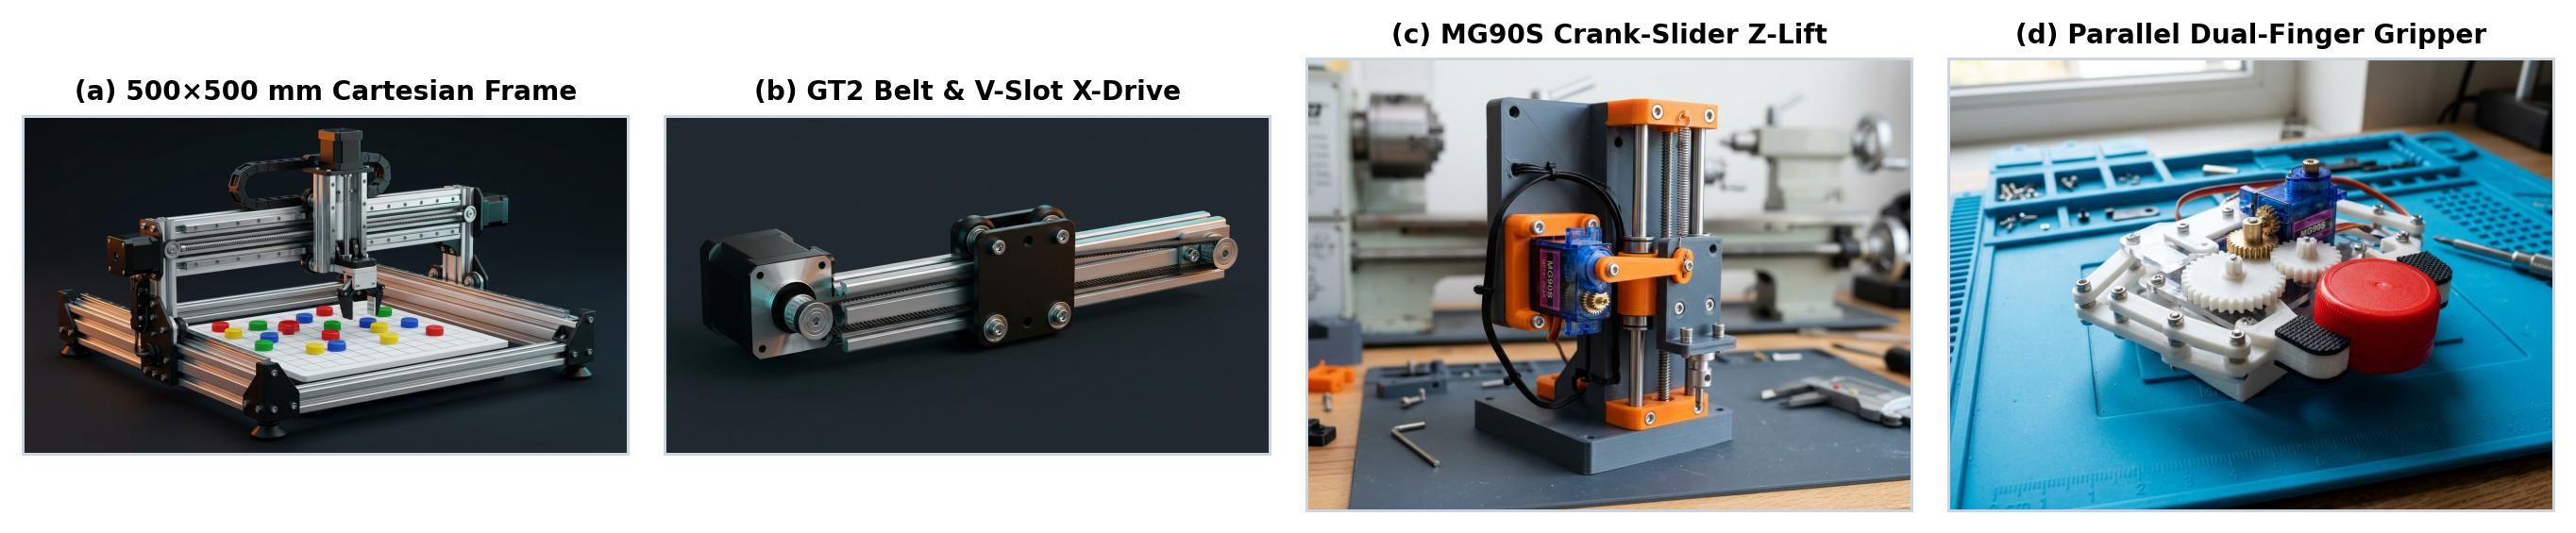
\includegraphics[width=\textwidth]{figures/fig_mechanical_cad.jpg}
  \caption{Mechanical CAD subsystem breakdown of CapSorter: (a)~rigid $500\times 500\times 500\text{ mm}$ 2020 V-slot moving-bridge Cartesian frame enclosing the $300\times 300\text{ mm}$ sorting workspace; (b)~GT2 $6\text{ mm}$ belt and 20-tooth pulley linear X-drive; (c)~guided crank-slider Z-axis lift driven by an MG90S metal-gear micro servo ($40\text{ mm}$ vertical stroke); and (d)~geared dual-finger parallel gripper ($36\text{ mm}$ open gap, $26\text{ mm}$ clamped width) fitted with high-friction TPU pads.}
  \label{fig:cad}
\end{figure*}

Two $40\text{ mm}$ NEMA~17 steppers ($200\text{ full steps/rev}$) drive 20-tooth GT2 timing pulleys ($p_{\mathrm{GT2}} = 2.0\text{ mm}$, $L_{\mathrm{rev}} = 40.0\text{ mm/rev}$) through TMC2208 drivers strapped for $m = 8$ microstepping (\texttt{MS1=MS2=GND}). The nominal commanded step scaling is:
\begin{equation}
  S_{\mathrm{nom}} = \frac{N_{\mathrm{full}} \cdot m}{N_{\mathrm{teeth}} \cdot p_{\mathrm{GT2}}} = \frac{200 \times 8}{20 \times 2.0} = 40.0\text{ steps/mm},
  \label{eq:step_scale}
\end{equation}
yielding a commanded resolution of $0.025\text{ mm/step}$ (distinct from physical bench accuracy, which depends on belt tension and backlash). To stay comfortably below the $\sim 4{,}000\text{ steps/s}$ timing ceiling of \texttt{AccelStepper} on a $16\text{ MHz}$ ATmega2560, firmware caps axis speed at $v_{\max} = 2{,}800\text{ steps/s}$ ($70.0\text{ mm/s}$) and acceleration at $a_{\max} = 6{,}000\text{ steps/s}^2$ ($150.0\text{ mm/s}^2$, $0.47\text{ s}$ ramp over $d_{\mathrm{ramp}} = v_{\max}^2 / a_{\max} = 32.67\text{ mm}$). The exact point-to-point move time for an independent simultaneous XY traverse $(\Delta x, \Delta y)$ is:
\begin{equation}
  T_{\mathrm{XY}}(\Delta x, \Delta y) = \max\!\big(T_{\mathrm{axis}}(|\Delta x|),\; T_{\mathrm{axis}}(|\Delta y|)\big),
  \label{eq:xy_move}
\end{equation}
where each single-axis trapezoidal/triangular profile obeys
\begin{equation}
  T_{\mathrm{axis}}(d) =
  \begin{cases}
    \dfrac{d}{v_{\max}} + \dfrac{v_{\max}}{a_{\max}}, & d \ge \dfrac{v_{\max}^2}{a_{\max}}, \\[8pt]
    2\sqrt{\dfrac{d}{a_{\max}}}, & d < \dfrac{v_{\max}^2}{a_{\max}}.
  \end{cases}
  \label{eq:trap_profile}
\end{equation}

The vertical Z-axis ($40\text{ mm}$ stroke) and parallel dual-finger gripper ($36\text{ mm}$ open inner gap, $26\text{ mm}$ clamped width, giving $\pm 3.0\text{ mm}$ nominal radial clearance around a $\varnothing 30\text{ mm}$ cap) are driven by two MG90S metal-gear servos through a PCA9685 16-channel 12-bit PWM controller over $400\text{ kHz}$ Fast-Mode I2C (re-asserted after \texttt{pca.begin()} alongside \texttt{Wire.setWireTimeout(3000, true)} to prevent AVR I2C bus lockup under stepper EMI). Hardware output enable (\texttt{PIN\_SERVO\_OE = Pin~9}, active-LOW) remains \texttt{HIGH} at boot and on hard faults to eliminate power-on twitching and uncommanded fault motion. To preserve strict coordinate-frame separation once physical toolhead offsets are measured, Mega firmware separates raw homed machine moves (\texttt{moveMachineToMm}, used for clear-FOV/home/failsafe $(0,0)$ parking and bench-measured external bin coordinates) from board-space cap moves (\texttt{moveBoardToMm}, adding \texttt{TOOL\_OFFSET\_X/Y\_MM} and verifying shifted machine travel bounds inside \texttt{isValidSingleTarget()}).

\subsection{Three-Branch Star-Ground Power Tree and Safety}
A single $12\text{ V}/10\text{ A}$ ($120\text{ W}$) SMPS supplies \textbf{three separate regulated branches sharing a common single-point star ground} (providing noise decoupling rather than galvanic isolation):
\begin{itemize}
  \item \textbf{Branch~A (Steppers, $12\text{ V}$ Fused):} Routed through Pole~1 of the dual-pole latching NC E-stop to both TMC2208 \texttt{VMOT} inputs with local $100\,\mu\text{F}$ low-ESR decoupling. Driver RMS coil current is calibrated using the ADI/Trinamic Rev~1.13 equation:
  \begin{equation}
    I_{\mathrm{RMS}} = \frac{0.325\text{ V}}{R_{\mathrm{sense}} + 0.03\,\Omega} \cdot \frac{1}{\sqrt{2}} \cdot \frac{V_{\mathrm{ref}}}{2.5\text{ V}},
    \label{eq:tmc_irms}
  \end{equation}
  yielding $I_{\mathrm{RMS}} \approx 0.75\text{ A}$ at $V_{\mathrm{ref}} = 1.15\text{ V}$ for standard $R_{\mathrm{sense}} = 0.11\,\Omega$ carriers (carrier SKU verification required prior to power-up).
  \item \textbf{Branch~B (Servos, $5\text{ V}/5\text{ A}$ Buck):} Also switched upstream by E-stop Pole~1, feeding \texttt{PCA9685 V+} with a $1{,}000\,\mu\text{F}$ bulk capacitor to absorb MG90S stall transients (noting that original TowerPro MG90S actuators are rated at $4.8\text{ V}$ nominal, requiring SKU verification).
  \item \textbf{Branch~C (Logic, $5\text{ V}/3\text{ A}$ Buck, Always-On):} Bypasses the E-stop directly from the $12\text{ V}$ SMPS (\cref{fig:architecture}, bottom strip) to power the Mega~2560 \texttt{5V} rail (not \texttt{VIN}, which requires $7\text{--}12\text{ V}$; protected against USB backfeed during flashing), PCA9685 \texttt{VCC}, and Teensy~4.1 \texttt{VIN} (V1) or Pi Zero~2~W \texttt{PWR IN} Micro-USB (V2, since the $3.5\text{ in}$ LCD covers Header Pins~1--26; combined V2 peak $\approx 1.4\text{ A}$ including the $\sim 160\text{ mA}$ LCD backlight and $\sim 30\text{ mA}$ CH9102/CP2102). Keeping logic energized during E-stop preserves fault telemetry and prevents Linux microSD corruption.
\end{itemize}

Because neither Teensy~4.1 nor $3.3\text{ V}$ CH9102/CP2102 USB-TTL modules guarantee full $5\text{ V}$ UART noise margin/tolerance against Mega~2560 \texttt{Serial1} ($V_{\mathrm{IH}}\ge 3.0\text{ V}$), a 4-channel bidirectional $3.3\text{ V}\leftrightarrow 5.0\text{ V}$ level shifter is mandatory on \emph{both} TX and RX lines (with V2 shifter \texttt{LV} fed from the converter's \texttt{3V3} pin and the converter's \texttt{+5V} pin left disconnected to prevent USB VBUS backfeed). Following ISO~13850 latching safety principles \cite{iso13850}, Pole~2 of the NC mushroom E-stop feeds Mega Pin~25 (\texttt{PIN\_ESTOP}, 2-sample debounced), latching \texttt{STATE\_HARD\_FAULT} (\texttt{0xEF}), driving \texttt{PIN\_STEPPER\_EN=HIGH} and \texttt{PIN\_SERVO\_OE=HIGH}, and requiring physical release plus explicit \texttt{CMD\_REARM\_HOME} (\texttt{0xB4}) and re-homing. Critically, Mega Pins~22 (\texttt{X}), 23 (\texttt{Y}), and 24 (\texttt{Z}) reside on ATmega2560 Port~A (\texttt{PA0--PA2}), which lacks hardware external or pin-change interrupts; firmware therefore polls all three NC limit switches every \texttt{loop()} iteration with 3-sample debouncing and executes a pre-homing $+10\text{ mm}$ backoff broken-wire check and post-homing $+3\text{ mm}$ switch-release verification within a $30\text{ s}$ seek timeout ($1.6\times$ margin over worst-case $370\text{ mm} / 20\text{ mm/s} = 18.5\text{ s}$).

% =========================================================================
% SECTION 4: VISION, CLOSED-LOOP PLANNING & PROTOCOL
% =========================================================================
\section{Embedded Vision, Planning, and Protocol}
\label{sec:method}

\begin{figure*}[t]
  \centering
  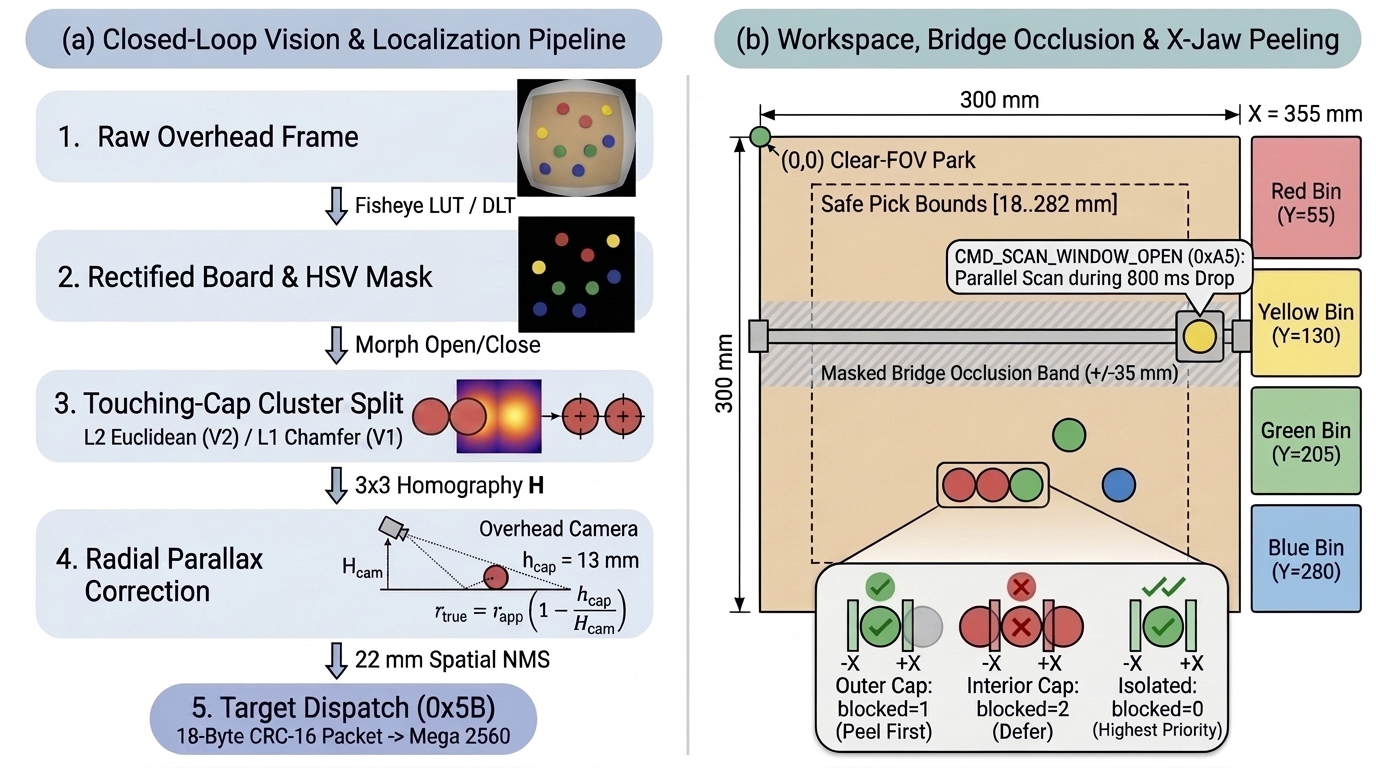
\includegraphics[width=\textwidth]{figures/fig_closed_loop_pipeline.jpg}
  \caption{CapSorter vision localization pipeline and closed-loop workspace geometry. \textbf{(a)}~Five-stage perceptual pipeline from raw wide-angle overhead capture through lens rectification, HSV masking, touching-cap distance-transform splitting ($L_2$ Euclidean in V2 / $L_1$ chamfer in V1), planar homography $\mathbf{H}$, and closed-form radial cap-height parallax compensation to 18-byte CRC-16 target dispatch. \textbf{(b)}~Continuous $300\times 300\text{ mm}$ open plywood workspace with safe pick bounds $[18,282]\text{ mm}$, four external bins at $X=355\text{ mm}$, the $\pm 35\text{ mm}$ horizontal Y-bridge occlusion band masked during parallel bin-side scanning (\texttt{0xA5}), and zoomed X-jaw footprint clearance peeling (\texttt{blocked=0} $\succ$ \texttt{blocked=1} $\succ$ \texttt{blocked=2}).}
  \label{fig:pipeline}
\end{figure*}

\subsection{Fail-Closed Calibration and Planar Homography}
To eliminate uncalibrated blind motion, both architectures enforce fail-closed startup guards: V1 halts motion unless \texttt{V1\_CALIBRATION\_VERIFIED == 1} and its 4-point homography is non-singular; V2 ships with an explicitly marked placeholder \texttt{calibration.npz} (\texttt{calibrated=False}) and raises \texttt{CalibrationError} whenever the archive is missing, uncalibrated, contains non-finite or singular matrices ($|\det \mathbf{H}| < 10^{-12}$), or mismatches the active \texttt{camera\_type} (\texttt{picamera2\_imx219} vs.\ \texttt{usb\_v4l2}) or frame resolution.

Intrinsic rectification supports both Brown--Conrady pinhole calibration \cite{zhang2000flexible} and the Kannala--Brandt equidistant fisheye model \cite{kannala2006generic}, where an incoming ray at angle $\theta = \arctan(r)$ projects radially as:
\begin{equation}
  \theta_d = \theta\!\left(1 + k_1\theta^2 + k_2\theta^4 + k_3\theta^6 + k_4\theta^8\right),
  \label{eq:fisheye}
\end{equation}
estimated from $N \ge 8$ checkerboard poses ($9\times 6$ inner corners, $25\text{ mm}$ squares, enforcing RMS reprojection error $\le 1.0\text{ px}$). Runtime undistortion uses precomputed \texttt{CV\_16SC2} lookup tables via \texttt{cv2.remap}. Rectified image coordinates $(u,v)$ map to $Z=0$ board millimeters $(x_{\mathrm{app}}, y_{\mathrm{app}})$ via a $3\times 3$ planar homography $\mathbf{H}$ ($h_{33}=1$) solved from the four board corner fiducials $(0,0), (300,0), (300,300), (0,300)\text{ mm}$ using OpenCV DLT (V2) or exact $8\times 8$ Gaussian elimination with partial pivoting (V1) \cite{hartley2004multiple}:
\begin{equation}
  \begin{aligned}
    \begin{bmatrix} w x_{\mathrm{app}} & w y_{\mathrm{app}} & w \end{bmatrix}^\top &= \mathbf{H} \begin{bmatrix} u & v & 1 \end{bmatrix}^\top, \\
    \mathbf{p}_{\mathrm{app}} = \begin{bmatrix} x_{\mathrm{app}} \\ y_{\mathrm{app}} \end{bmatrix} &= \frac{1}{w}\begin{bmatrix} h_{11}u + h_{12}v + h_{13} \\ h_{21}u + h_{22}v + h_{23} \end{bmatrix}.
  \end{aligned}
  \label{eq:homography}
\end{equation}

\subsection{Radial Cap-Height Parallax Compensation}
Because $\mathbf{H}$ maps points strictly on the $Z=0$ plywood surface while a bottle cap's colored top face lies at elevation $h_{\mathrm{cap}} \approx 13.0\text{ mm}$, perspective projection from an overhead camera mounted at height $H_{\mathrm{cam}}$ above the board shifts the apparent centroid radially outward from the projected optical center $\mathbf{c}_{\mathrm{opt}} = \mathbf{H}[c_x, c_y, 1]^\top$ (\cref{fig:pipeline}a, Stage~4). By similar triangles, an object at true radial distance $r_{\mathrm{true}} = \|\mathbf{p}_{\mathrm{true}} - \mathbf{c}_{\mathrm{opt}}\|_2$ projects to $r_{\mathrm{app}} = r_{\mathrm{true}} \cdot H_{\mathrm{cam}} / (H_{\mathrm{cam}} - h_{\mathrm{cap}})$, producing an uncompensated radial error:
\begin{equation}
  \Delta r_{\mathrm{parallax}} = r_{\mathrm{app}} - r_{\mathrm{true}} = r_{\mathrm{true}} \cdot \frac{h_{\mathrm{cap}}}{H_{\mathrm{cam}} - h_{\mathrm{cap}}}.
  \label{eq:parallax_err}
\end{equation}
At $H_{\mathrm{cam}}=200\text{ mm}$ and board-corner radius $r_{\mathrm{true}}=175\text{ mm}$, \cref{eq:parallax_err} yields $\Delta r = 12.17\text{ mm}$—over $4\times$ the gripper's $\pm 3.0\text{ mm}$ radial clearance. Both V1 and V2 invert this geometry analytically whenever $H_{\mathrm{cam}} > h_{\mathrm{cap}} > 0$:
\begin{equation}
  \mathbf{p}_{\mathrm{true}} = \mathbf{c}_{\mathrm{opt}} + \left(1 - \frac{h_{\mathrm{cap}}}{H_{\mathrm{cam}}}\right)\!\left(\mathbf{p}_{\mathrm{app}} - \mathbf{c}_{\mathrm{opt}}\right).
  \label{eq:parallax_comp}
\end{equation}

\subsection{HSV Segmentation and Touching-Cap Splitting}
Following perceptual HSV conversion \cite{smith1978color}, pixels are partitioned into four calibrated color classes (Red dual-wrap $H\in[0,10]\cup[168,180]$, Yellow $[18,35]$, Green $[38,85]$, Blue $[98,132]$ on the $[0,180]$ OpenCV hue scale) with saturation/value floors rejecting matte plywood and specular glare. Morphological opening/closing ($5\times 5$ elliptical kernels in V2; $3\times 3$ majority-4/close-5 integer filter in V1) removes speckle and seals glare holes. Single isolated caps satisfy area and circularity bounds $C = 4\pi A / P^2 \ge 0.72$ (V2) or $0.70$ (V1) and yield moment centroids directly \cite{suzuki1985topological}.

Whenever two or more same-color caps touch, their merged silhouette violates the single-cap area ceiling or circularity threshold and triggers distance-transform peak splitting:
\begin{itemize}
  \item \textbf{V1 Bare-Metal $L_1$ Chessboard Chamfer Splitter:} Within a bounded ROI ($\le 160\times 160\text{ px}$, $25.0\text{ KiB}$ in static \texttt{splitDistMap}), Teensy executes a forward-and-backward $3\times 3$ chessboard chamfer transform \cite{borgefors1986distance}, extracts local maxima over a $7\times 7$ neighborhood ($\text{val} \ge 6\text{ px}$), and deduplicates candidates via area-sorted insertion sort + greedy spatial non-maximum suppression (NMS) at $d_{\mathrm{NMS}} = 22.0\text{ mm}$.
  \item \textbf{V2 Gap-Preserving $L_2$ Euclidean Splitter:} To preserve small triangular plywood voids enclosed inside 3-cap or 4-cap clusters, V2 intersects the filled contour ROI with the morphologically opened binary mask \texttt{mask\_opened} before computing the exact $5\times 5$ Euclidean distance transform \texttt{cv2.DIST\_L2} \cite{felzenszwalb2012distance}, smoothing with a $5\times 5$ Gaussian ($\sigma=1.0$), detecting local peaks via elliptical dilation ($k \approx 0.55\,R_{\mathrm{px}}$) above $0.45\,R_{\mathrm{px}}$, suppressing sub-peaks within $1.25\,R_{\mathrm{px}}$, and applying $22.0\text{ mm}$ spatial NMS.
\end{itemize}

\subsection{Pipelined Bin-Side Re-Imaging and Clearance Peeling}
\label{sec:closed_loop}
\Cref{alg:closed_loop} formalizes CapSorter's closed-loop sorting controller, illustrated spatially in \cref{fig:pipeline}b.

\begin{algorithm}[t]
\caption{CapSorter Closed-Loop Pipelined Bin-Side Sorting}
\label{alg:closed_loop}
\small
\begin{algorithmic}[1]
\REQUIRE Validated calibration $(\mathbf{K},\mathbf{D},\mathbf{H},H_{\mathrm{cam}})$; Mega in \texttt{READY} at $(0,0)$
\STATE $\mathcal{R} \leftarrow \emptyset$ (retry records), $\mathcal{Q} \leftarrow \emptyset$ (quarantined spots)
\STATE Capture Scan~\#0 at $(0,0)$; $\mathcal{C} \leftarrow \textsc{Detect}(I_0, \varnothing)$
\STATE $c^\star \leftarrow \textsc{SelectNext}(\mathcal{C}, (0,0), \mathcal{R}, \mathcal{Q})$
\WHILE{$c^\star \neq \varnothing$ \textbf{and} $\text{cycles} < 200$}
  \STATE Send 18B \texttt{0x5B} CRC-16 packet for $c^\star$; await \texttt{CMD\_BATCH\_ACK}
  \STATE $(x_b, y_b) \leftarrow \textsc{BinCoord}(c^\star.\text{color})$; $c_{\mathrm{next}} \leftarrow \varnothing$; $\text{eval} \leftarrow \text{false}$
  \WHILE{not received \texttt{CMD\_AWAIT\_NEXT} (\texttt{0xA6})}
    \STATE Emit \texttt{0xF0} heartbeat every $250\text{ ms}$; abort on fault/timeout
    \IF{received \texttt{CMD\_SCAN\_WINDOW\_OPEN} (\texttt{0xA5})}
      \STATE \COMMENT{\emph{Runs in parallel with Mega's $800\text{ ms}$ bin-drop dwell}}
      \STATE Capture fresh $I_k$; $\mathcal{C}_k \leftarrow \textsc{Detect}(I_k, y_b)$
      \STATE $\text{eval} \leftarrow \textsc{UpdateRetry}(c^\star, \mathcal{C}_k, \mathcal{R}, \mathcal{Q}, y_b)$
      \STATE $c_{\mathrm{next}} \leftarrow \textsc{SelectNext}(\mathcal{C}_k, (x_b, y_b), \mathcal{R}, \mathcal{Q})$
    \ENDIF
  \ENDWHILE
  \IF{$c_{\mathrm{next}} \neq \varnothing$}
    \STATE $c^\star \leftarrow c_{\mathrm{next}}$ \COMMENT{\emph{Direct bin-to-cap dispatch (no home park)}}
  \ELSE
    \STATE Send \texttt{CMD\_PARK\_FOR\_SCAN} (\texttt{0xB5}); await \texttt{0xA6} at $(0,0)$
    \STATE Capture unoccluded $I_v$; $\mathcal{C}_v \leftarrow \textsc{Detect}(I_v, \varnothing)$
    \IF{not $\text{eval}$}
      \STATE $\textsc{UpdateRetry}(c^\star, \mathcal{C}_v, \mathcal{R}, \mathcal{Q}, \varnothing)$
    \ENDIF
    \STATE $c^\star \leftarrow \textsc{SelectNext}(\mathcal{C}_v, (0,0), \mathcal{R}, \mathcal{Q})$
  \ENDIF
\ENDWHILE
\STATE Send \texttt{CMD\_FINISH\_SESSION} (\texttt{0xB6}); await \texttt{CMD\_BATCH\_COMPLETE}
\end{algorithmic}
\end{algorithm}

\paragraph{X-Axis Jaw-Footprint Clearance-First Peeling.}
When descending onto target cap $i$ at $(x_i, y_i)$, the open parallel gripper jaws occupy two physical footprints along the X-axis:
\begin{equation}
  \begin{aligned}
    \mathcal{B}_i^{-} &= [x_i - W_{\mathrm{out}},\; x_i - W_{\mathrm{in}}] \times [y_i - W_{\perp},\; y_i + W_{\perp}], \\
    \mathcal{B}_i^{+} &= [x_i + W_{\mathrm{in}},\; x_i + W_{\mathrm{out}}] \times [y_i - W_{\perp},\; y_i + W_{\perp}],
  \end{aligned}
  \label{eq:jaw_boxes}
\end{equation}
where $W_{\mathrm{in}}=18.0\text{ mm}$, $W_{\mathrm{out}}=26.0\text{ mm}$, and $W_{\perp}=10.0\text{ mm}$. A neighboring cap $j \neq i$ (including out-of-bounds or quarantined caps, which remain physical obstacles) blocks jaw side $s \in \{-,+\}$ if its expanded disk of radius $R_{\mathrm{chk}} = R_{\mathrm{cap}} + 1.5 = 16.5\text{ mm}$ intersects $\mathcal{B}_i^{s}$ under exact 2D circle--rectangle distance:
\begin{equation}
  \begin{aligned}
    \mathrm{blocked}(i) &= \mathbb{I}\!\left(\exists j\neq i:\, d(\mathbf{p}_j, \mathcal{B}_i^{-}) < R_{\mathrm{chk}}\right) \\
                        &\quad + \mathbb{I}\!\left(\exists j\neq i:\, d(\mathbf{p}_j, \mathcal{B}_i^{+}) < R_{\mathrm{chk}}\right),
  \end{aligned}
  \label{eq:blocked}
\end{equation}
taking values in $\{0,1,2\}$. Valid unquarantined targets inside safe pick bounds are ranked lexicographically by:
\begin{equation}
  \begin{aligned}
    c^\star = \arg\min_{i \in \mathcal{V}} \Big(& r_i,\; \mathrm{blocked}(i),\; \|\mathbf{p}_i - \mathbf{p}_{\mathrm{cur}}\|_2, \\
                                                & -\min_{j\neq i}\|\mathbf{p}_i - \mathbf{p}_j\|_2 \Big),
  \end{aligned}
  \label{eq:selector}
\end{equation}
where $r_i \in \{0,1\}$ defers previously missed spots. This peels dense clusters strictly outside-in (\texttt{blocked=0} isolated caps first, then \texttt{blocked=1} perimeter caps, avoiding \texttt{blocked=2} double-sided pinches) while minimizing travel from the current bin.

\paragraph{Pipelined Bin-Side Latency Hiding, Occlusion Masking, and Finite Termination.}
Upon reaching bin $(355.0, y_b)$, the Mega pauses $t_{\mathrm{settle}} = 120\text{ ms}$ in \texttt{STATE\_BIN\_SETTLE} with Z raised so belt vibration damps, then emits \texttt{CMD\_SCAN\_WINDOW\_OPEN} (\texttt{0xA5}) and immediately begins its $t_{\mathrm{drop}} = 800\text{ ms}$ bin-drop sequence (\texttt{LOWER\_BIN} $250\text{ ms}$ + \texttt{RELEASE\_CAP} $250\text{ ms}$ + \texttt{RETRACT\_Z} $300\text{ ms}$). Total single-cap cycle duration is therefore:
\begin{equation}
  T_{\mathrm{cycle}} = T_{\mathrm{XY}}^{\mathrm{to\text{-}cap}} + t_{\mathrm{pick}} + T_{\mathrm{XY}}^{\mathrm{to\text{-}bin}} + t_{\mathrm{settle}} + \max\!\left(t_{\mathrm{drop}},\; T_{\mathrm{scan}}\right),
  \label{eq:pipelined_cycle}
\end{equation}
with $t_{\mathrm{pick}} = 350 + 300 + 350 = 1{,}000\text{ ms}$. Because V2's $T_{\mathrm{scan}} \approx 45\text{ ms} \ll 800\text{ ms}$, closed-loop re-imaging adds \emph{zero} vision stall overhead on V2 (compared to $+0.91\text{ s}$ overhang on V1 where $T_{\mathrm{scan}} \approx 1.71\text{ s}$). During a bin-side scan, the moving Y-bridge crosses the workspace at $Y = y_b$; detections inside $|y - y_b| \le 35.0\text{ mm}$ are masked out, and retry evaluation is deferred if the just-picked cap lay in that band. When no unmasked graspable cap remains, the host sends \texttt{CMD\_PARK\_FOR\_SCAN} (\texttt{0xB5}) to park at $(0,0)$ and performs a full unobstructed verification scan before terminating with \texttt{CMD\_FINISH\_SESSION} (\texttt{0xB6}). Finally, if a same-color cap remains within $14.0\text{ mm}$ of $c^\star$ on an unoccluded scan for $3$ consecutive attempts, the coordinate is inserted into quarantine set $\mathcal{Q}$.

\paragraph{Proposition 1 (Bounded Finite Termination).}
\emph{Given $N_0 \le 100$ initial caps within safe reachability bounds, a finite quarantine radius $R_{\mathrm{miss}} = 14.0\text{ mm}$, retry limit $K_{\max} = 3$, and hard safety ceiling $C_{\max} = 200$, \cref{alg:closed_loop} terminates in at most $\min(K_{\max} N_0,\; C_{\max})$ pick cycles even under persistent mechanical sticking or grasp failure.}
\emph{Proof sketch.} Each pick cycle either removes a cap from the board (strictly decreasing active cap count) or increments its retry counter inside an unoccluded scan (or following \texttt{CMD\_PARK\_FOR\_SCAN}). Once $K_{\max}=3$ attempts occur without displacing a cap beyond $R_{\mathrm{miss}}$, that coordinate enters $\mathcal{Q}$ and is excluded from $\mathcal{V}$ for the session remainder; hence each of the $N_0$ caps can trigger at most $3$ dispatches, bounded globally by $C_{\max}=200$. $\square$

\subsection{CRC-16/CCITT Wire Protocol and Comms-Loss FSM}
All inter-controller messages are strictly typed in shared header \texttt{packet\_protocol.h} (\cref{tab:protocol}). Closed-loop targets use an 18-byte packed frame \texttt{[0x5B][CapTarget 15B][CRC16 2B]} ($\text{tx time} = 1.56\text{ ms}$ at $115{,}200\text{ baud}$), verified by CRC-16/CCITT-FALSE (polynomial \texttt{0x1021}, initial value \texttt{0xFFFF}, check vector \texttt{"123456789"} $\to$ \texttt{0x29B1}) \cite{koopman2004cyclic}; legacy multi-cap batches (\texttt{0x5A}, up to $100$ caps, paced in $32\text{ B}$ chunks with $2\text{ ms}$ gaps to protect the Mega's $64\text{ B}$ RX FIFO) remain supported for backward compatibility.

\Cref{fig:safety_fsm}a illustrates Mega's deterministic motion and safety FSM. During active motion, the Mega monitors \texttt{CMD\_HEARTBEAT\_PING} (\texttt{0xF0}, nominal $250\text{ ms}$ cadence). If $>1{,}200\text{ ms}$ elapses without a ping, \texttt{executeSafeCommsLossPolicy()} latches \texttt{commsFaultLatched=true} and emits \texttt{CMD\_RECOVERY\_HALT} (\texttt{0xEE}). If a single scanned cap is already mid-cycle (\texttt{inActiveCapCycle}), the Mega finishes depositing \emph{only} that active cap into its assigned bin (canceling bin-side scans and all subsequent targets), transitions to \texttt{STATE\_FAILSAFE\_PARKING} to return cleanly to $(0,0)$, de-energizes \texttt{PIN\_STEPPER\_EN=HIGH}, and latches \texttt{STATE\_FAILSAFE\_HALT}. Unlike unsafe auto-resume schemes, returning UART pings can never re-initiate motion; explicit operator \texttt{CMD\_REARM\_HOME} (\texttt{0xB4}) and full re-homing are mandatory. Both V1 and V2 flush stale queued RX fault bytes prior to issuing \texttt{CMD\_REARM\_HOME} or polling \texttt{CMD\_QUERY\_STATUS} so multiple \texttt{0xEE} bytes emitted during a comms-loss park cannot poison post-rearm readiness confirmation.

\begin{table}[t]
  \centering
  \resizebox{\columnwidth}{!}{%
  \begin{tabular}{@{}llcl@{}}
    \toprule
    \textbf{Opcode / Frame} & \textbf{Hex} & \textbf{Dir.} & \textbf{Function \& Integrity Guard} \\
    \midrule
    \texttt{CMD\_QUERY\_STATUS} & \texttt{0xB0} & H$\to$M & Poll Mega readiness before start \\
    \texttt{CMD\_STATUS\_RDY/BSY/FLT} & \texttt{0xB1--B3} & M$\to$H & Ready / homing-busy / fault latched \\
    \texttt{PROTOCOL\_SINGLE} & \texttt{0x5B} & H$\to$M & 18\,B target + CRC-16 + safe bounds \\
    \texttt{CMD\_BATCH\_ACK / NACK} & \texttt{0xA1/A2} & M$\to$H & Valid CRC / reject \& retry ($\le 3\times$) \\
    \texttt{CMD\_SCAN\_WINDOW\_OPEN} & \texttt{0xA5} & M$\to$H & Settled $120\text{ ms}$; start parallel scan \\
    \texttt{CMD\_PROGRESS / AWAIT} & \texttt{0xA4/A6} & M$\to$H & Reset $25\text{ s}$ stall / ready for next \\
    \texttt{CMD\_PARK\_FOR\_SCAN} & \texttt{0xB5} & H$\to$M & Park $(0,0)$ for unoccluded FOV \\
    \texttt{CMD\_FINISH / COMPLETE} & \texttt{0xB6/A3} & H$\leftrightarrow$M & Park $(0,0)$ $\to$ \texttt{STATE\_IDLE} \\
    \texttt{CMD\_HEARTBEAT\_PING} & \texttt{0xF0} & H$\to$M & $250\text{ ms}$ keep-alive ($1.2\text{ s}$ WDT) \\
    \texttt{CMD\_RECV / HARD\_FLT} & \texttt{0xEE/EF} & M$\to$H & Comms-loss park / E-stop or NC trip \\
    \texttt{CMD\_REARM\_HOME} & \texttt{0xB4} & H$\to$M & Operator clear + full re-home \\
    \bottomrule
  \end{tabular}}
  \caption{Core binary UART1 protocol opcodes (\texttt{packet\_protocol.h}, $115{,}200\text{ baud}$, 8N1) shared identically across V1 and V2 (H = Vision Host, M = Mega~2560).}
  \label{tab:protocol}
\end{table}

% =========================================================================
% SECTION 5: EXPERIMENTAL EVALUATION & VERIFICATION
% =========================================================================
\section{Experimental Evaluation and Verification}
\label{sec:experiments}

\subsection{Verification Harness and Automated Test Suite}
Because physical bench assembly and hardware SKU sign-off remain ongoing (\cref{sec:limitations}), all quantitative results below are obtained via reproducible Software-in-the-Loop (SIL), synthetic-optics, and analytical kinematic benchmarks directly executing \texttt{pi\_zero\_vision.py}, \texttt{lcd\_hud.py}, and \texttt{fisheye\_calibrate.py}, paired with bit-exact mirrors of \texttt{teensy\_vision.cpp} (including RGB565 5-6-5 quantization, integer HSV, $3\times 3$ morphological filtering, and two-pass chamfer splitting) and \texttt{mega\_motion.ino}'s exact trapezoidal \texttt{AccelStepper} dynamics (\cref{eq:xy_move,eq:trap_profile}).

First, the repository's 36-test automated verification and SIL suite (\texttt{firmware/tests/test\_validation.py}) executes in $<5\text{ s}$ with \textbf{36/36 tests passing}, verifying: (i)~19-opcode C/Python parity and exact struct packing (\texttt{6\,B} header, \texttt{15\,B} target, \texttt{18\,B} single frame); (ii)~fail-closed rejection of shipped placeholder, missing, camera-mismatched, resolution-mismatched, and geometrically invalid fiducial calibrations (bow-tie, counter-clockwise, rotated, out-of-bounds, sliver, and bad interior check points); (iii)~100-cap dynamic supervision exceeding $850\text{ s}$ ($>3{,}000$ heartbeats), guarded V2 background heartbeat continuity across slow captures + intentional stall cutoff, and immediate fault halting; (iv)~mid-cycle bumped-neighbor re-acquisition (a $(+32,-24)\text{ mm}$ displacement re-acquired within $<2.5\text{ mm}$), bridge-occluded cap reveal via clear-FOV parking, and 3-attempt stuck-cap quarantine (without falsely incrementing sorted bin counts); (v)~USB-TTL serial auto-detection (\texttt{/dev/capsorter\_mega} via \texttt{udev} rules for WCH \texttt{1a86} / CP2102 \texttt{10c4}), thread-safe UART closure/reconnect, and stride/bitfield-aware $480\times 320$ 16/32-bpp SPI LCD HUD kinematic interpolation, rendering, and touch hit-testing; (vi)~full closed-loop end-to-end SIL runs pairing \texttt{PiZeroVisionController} and \texttt{CapSorterLCDHUD} against a discrete-time \texttt{SimulatedMega2560} FSM verifying non-zero \texttt{TOOL\_OFFSET} $(16.5,11.0)\text{ mm}$ machine/board frame separation, mid-cap UART-cut active-cycle completion + $(0,0)$ park + halt + RX-flushed \texttt{CMD\_REARM\_HOME} recovery, and clean mid-session LCD pause; (vii)~step-bounded homing, timed switch debouncing ($4\text{ ms}$ E-stop / $8\text{ ms}$ limits), wired \texttt{HAS\_GRIP\_SENSOR} guards, V1 BFS overflow rejection + \texttt{EXEC\_CAPTURE\_FAULT} + operator \texttt{REARM}, Stage~3 jog safety interlocks, and smoke execution of all 8 staged hardware bring-up utilities (\texttt{firmware/bringup/}); and (viii)~verbatim firmware/web-vault synchronization across all 9 HTML blocks and zero unsubstantiated safety claims. Second, CRC-16/CCITT-FALSE fault injection across $15{,}000$ corrupted 15-byte payloads ($5{,}000$ single-bit, $5{,}000$ double-bit, and $5{,}000$ random $3\text{--}16\text{ bit}$ bursts) achieved \textbf{100.00\% (15,000/15,000)} corruption rejection.

\subsection{Calibration, Undistortion, and Radial Parallax}
\Cref{tab:calibration} and \cref{fig:calibration_parallax}a evaluate planar localization across an $8\times 8$ ground-truth workspace grid ($N=64$ positions spanning $[30,270]^2\text{ mm}$) using 14 full-FOV synthetic checkerboard poses ($9\times 6$ inner corners, $25\text{ mm}$ squares). On V2's $160^\circ$ fisheye lens, calibrated Kannala--Brandt rectification achieves $\text{RMS} = 0.1039\text{ px}$ and reduces mean localization error by \textbf{24.4$\times$} ($7.15\to 0.29\text{ mm}$) and maximum corner error by \textbf{40.4$\times$} ($20.40\to 0.51\text{ mm}$)—converting guaranteed corner grasp misses into sub-millimeter precision well inside the $\pm 3.0\text{ mm}$ jaw half-clearance. V2 pinhole calibration similarly cuts error $3.2\times$ to $0.29\text{ mm}$ mean ($0.42\text{ mm}$ max, $\text{RMS}=0.0713\text{ px}$), while V1 QVGA 4-point DLT achieves $0.43\text{ mm}$ mean ($0.64\text{ mm}$ max) under rectilinear optics with machine-precision corner residual ($5.68\times 10^{-14}\text{ mm}$).

\paragraph{Calibration FOV-Coverage Finding.}
During ablation, restricting fisheye checkerboard capture to 10 narrow central poses produced low nominal RMS ($0.113\text{ px}$) yet caused higher-order equidistant terms ($k_3\theta^7, k_4\theta^9$) to diverge at extreme peripheral $\theta$, degrading edge localization to $\text{P95} = 30.15\text{ mm}$ ($45/64$ detected). Expanding capture to 14 poses covering all four corners completely stabilized all coefficients ($64/64$, $\max = 0.51\text{ mm}$), demonstrating why bench calibration SOPs must mandate corner-spanning checkerboard coverage.

\begin{table*}[t]
  \centering
  \resizebox{\textwidth}{!}{%
  \begin{tabular}{@{}lccccccc@{}}
    \toprule
    \textbf{Pipeline / Lens Model} & \textbf{Resolution} & \textbf{Scale (px/mm)} & \textbf{Calib. RMS} & \textbf{Unrect. Mean / Max} & \textbf{Rect. Mean / Med / P95 / Max} & \textbf{Detected} & \textbf{Vision Latency} \\
    \midrule
    V1 4-Pt DLT (rectilinear) & $320{\times}240$ & $0.76 \times 0.69$ & $5.68{\times}10^{-14}\text{ mm}$ & --- & $0.43 / 0.44 / 0.64 / 0.64\text{ mm}$ & 64 / 64 & $\sim 40\text{ ms}$ (M7 est.) \\
    V2 Pinhole (USB V4L2) & $640{\times}480$ & $1.45$ & $0.0713\text{ px}$ & $0.93 / 2.76\text{ mm}$ & $\mathbf{0.29} / \mathbf{0.29} / \mathbf{0.39} / \mathbf{0.42}\text{ mm}$ & 64 / 64 & $3.85\text{ ms}$ (host) / $\sim 25\text{ ms}$ (Pi) \\
    V2 $160^\circ$ Fisheye (IMX219 CSI) & $640{\times}480$ & $1.20$ & $0.1039\text{ px}$ & $7.15 / 20.40\text{ mm}$ & $\mathbf{0.29} / 0.30 / 0.49 / 0.51\text{ mm}$ & 64 / 64 & $4.11\text{ ms}$ (host) / $\sim 25\text{ ms}$ (Pi) \\
    \bottomrule
  \end{tabular}}
  \caption{Planar localization error across an $8\times 8$ ground-truth workspace grid ($N=64$ points) comparing V1 QVGA DLT against V2 pinhole and $160^\circ$ fisheye pipelines calibrated with 14 full-FOV checkerboard poses.}
  \label{tab:calibration}
\end{table*}

\begin{figure*}[t]
  \centering
  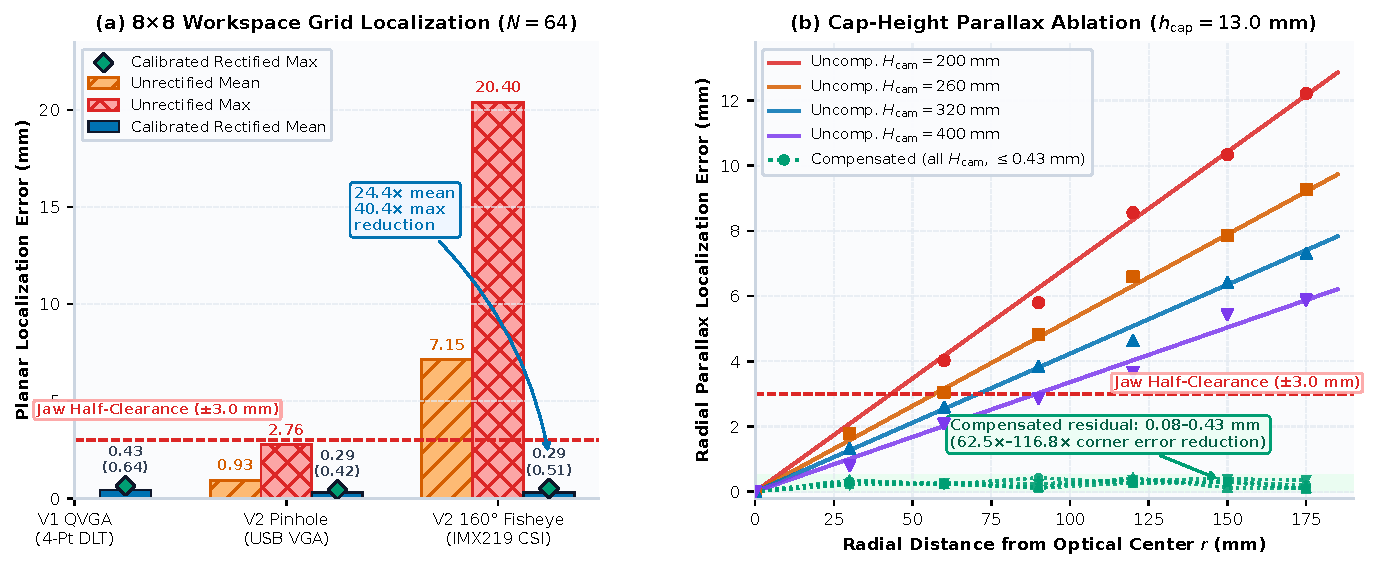
\includegraphics[width=\textwidth]{figures/fig_parallax_and_calibration.pdf}
  \caption{Optical localization and radial parallax verification. \textbf{(a)}~Planar localization error across $N=64$ grid positions before and after intrinsic calibration, showing $24.4\times$ mean ($40.4\times$ max) error reduction on the $160^\circ$ IMX219 fisheye lens. \textbf{(b)}~Radial cap-height parallax error ($h_{\mathrm{cap}}=13.0\text{ mm}$) versus radial offset $r$ across four mounting heights $H_{\mathrm{cam}}\in\{200,260,320,400\}\text{ mm}$: solid lines denote analytical \cref{eq:parallax_err}, markers denote uncompensated vision measurements, and dotted green curves show compensated residuals ($\le 0.43\text{ mm}$ across all heights).}
  \label{fig:calibration_parallax}
\end{figure*}

\Cref{fig:calibration_parallax}b quantifies radial cap-height parallax ($h_{\mathrm{cap}}=13.0\text{ mm}$) along the $45^\circ$ board diagonal across $H_{\mathrm{cam}} \in \{200, 260, 320, 400\}\text{ mm}$. Measured uncompensated errors track analytical \cref{eq:parallax_err} closely, reaching $12.22\text{ mm}$ ($H_{\mathrm{cam}}=200\text{ mm}$), $9.27\text{ mm}$ ($260\text{ mm}$), $7.31\text{ mm}$ ($320\text{ mm}$), and $5.88\text{ mm}$ ($400\text{ mm}$) at $r=175\text{ mm}$—exceeding $\pm 3.0\text{ mm}$ jaw tolerance at every practical enclosure height. Enabling \cref{eq:parallax_comp} collapses the residual to $0.08\text{--}0.43\text{ mm}$ across all radii and heights (a \textbf{62.5$\times$--116.8$\times$} reduction at $r=175\text{ mm}$).

\subsection{Touching Same-Color Cluster Separation}
\Cref{tab:clusters} and \cref{fig:clusters} benchmark touching same-color cap separation at $30.5\text{ mm}$ center spacing (matching tolerance $4.5\text{ mm}$). Naive contour centroiding achieves $100\%$ F1 only on isolated caps and collapses to \textbf{0.0\% F1} on every touching configuration because merged blobs report false centroids lying on cap boundaries or empty gaps. V1's $25.0\text{ KiB}$ integer $L_1$ chessboard chamfer splitter recovers $100.0\%$ F1 on pairs, equilateral triangles, and $2\times 2$ quads ($1.00\text{--}2.54\text{ mm}$ mean error) and $82.4\%$ F1 ($7/9$ TP) on the dense $3\times 3$ cluster, where QVGA's coarse $0.76\text{ px/mm}$ pitch causes integer chamfer plateaus to merge two adjacent blue peaks (\cref{fig:clusters}c). V2's VGA $L_2$ Euclidean distance transform with interior-gap mask preservation achieves \textbf{100.0\% F1 across all five benchmarks} with sub-millimeter centroid error ($0.12\text{--}0.79\text{ mm}$; \cref{fig:clusters}a--b).

\begin{table}[t]
  \centering
  \resizebox{\columnwidth}{!}{%
  \begin{tabular}{@{}lcccc@{}}
    \toprule
    \textbf{Cluster Benchmark} & \textbf{GT} & \textbf{Naive F1} & \textbf{V1 Chamfer F1 (Err)} & \textbf{V2 $L_2$ F1 (Err)} \\
    \midrule
    Isolated 4 Caps & 4 & 100.0\% & 100.0\% ($0.60\text{ mm}$) & \textbf{100.0\% ($0.32\text{ mm}$)} \\
    Touching Pairs ($30.5\text{ mm}$) & 4 & 0.0\% & 100.0\% ($1.00\text{ mm}$) & \textbf{100.0\% ($0.12\text{ mm}$)} \\
    2$\times$ Equilateral Triangles & 6 & 0.0\% & 100.0\% ($2.54\text{ mm}$) & \textbf{100.0\% ($0.28\text{ mm}$)} \\
    2$\times$2 Quad Cluster & 4 & 0.0\% & 100.0\% ($2.04\text{ mm}$) & \textbf{100.0\% ($0.29\text{ mm}$)} \\
    Dense 3$\times$3 (5R + 4B) & 9 & 0.0\% & 82.4\% ($1.61\text{ mm}$) & \textbf{100.0\% ($0.79\text{ mm}$)} \\
    \bottomrule
  \end{tabular}}
  \caption{Touching same-color cap separation F1 score and mean centroid localization error across five geometric benchmarks.}
  \label{tab:clusters}
\end{table}

\begin{figure*}[t]
  \centering
  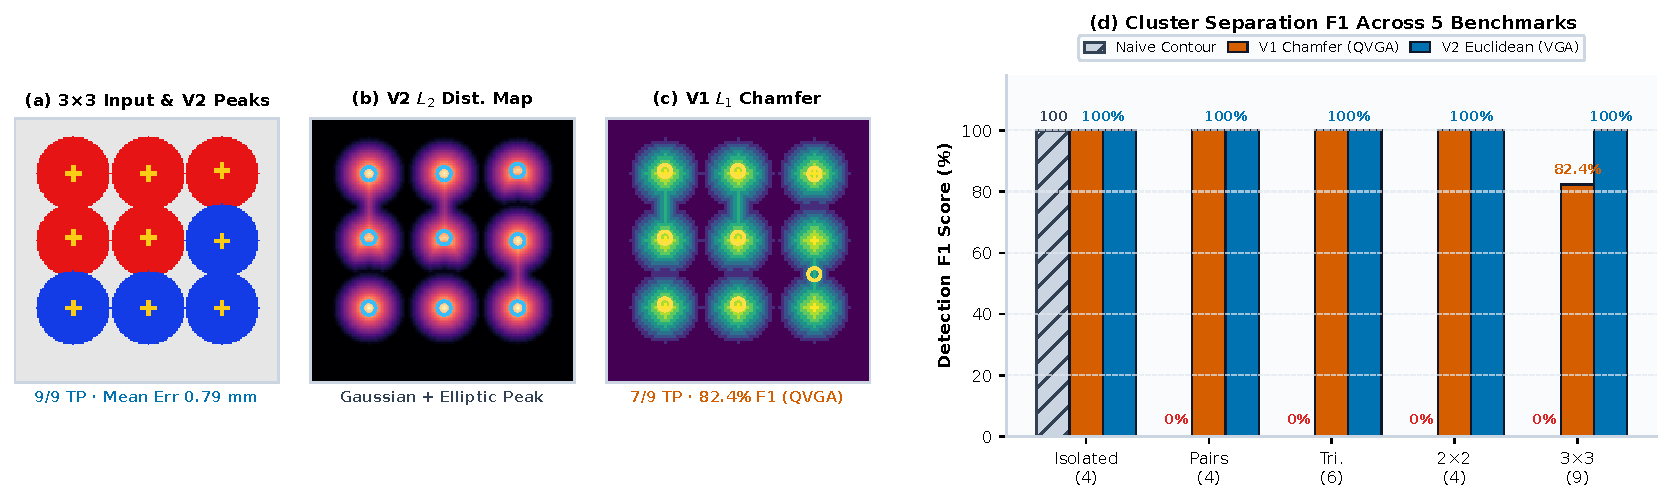
\includegraphics[width=\textwidth]{figures/fig_cluster_splitting_visual.pdf}
  \caption{Live firmware visualization and quantitative benchmark for touching same-color cap separation. \textbf{(a)}~Dense $3\times 3$ touching cluster (5 Red, 4 Blue at $30.5\text{ mm}$ spacing) with V2 detected centroids ($9/9$ TP, $0.79\text{ mm}$ mean error). \textbf{(b)}~V2 gap-preserving $L_2$ Euclidean distance map with circular peak markers. \textbf{(c)}~V1 QVGA $L_1$ chessboard chamfer map ($7/9$ TP, $82.4\%$ F1 due to coarse pixel discretization). \textbf{(d)}~F1 comparison across all five benchmarks showing Naive contour failure ($0\%$) versus V1 and V2 splitting.}
  \label{fig:clusters}
\end{figure*}

\subsection{Monte Carlo Closed-Loop Policy Ablation and Throughput}
To quantify closed-loop resilience against physical open-plate neighbor bumps, we ran a deterministic Monte Carlo SIL ablation over $N=50$ randomized cluttered boards ($12\text{ caps/board}$, $600\text{ caps}$ total), each seeded with tight 3-cap horizontal clusters ($31.5\text{ mm}$ spacing) plus scattered caps. Whenever descending open jaws intersect a neighbor disk ($R_{\mathrm{chk}}=16.5\text{ mm}$), the neighbor is nudged outward by $12\text{--}22\text{ mm}$; grasps succeed if the target cap sits within $\pm 7.5\text{ mm}$ of commanded $(x,y)$. \Cref{tab:ablation} and \cref{fig:ablation}a compare four policies under exact Mega~2560 kinematics (\cref{eq:xy_move,eq:trap_profile,eq:pipelined_cycle}):

\begin{table*}[t]
  \centering
  \resizebox{\textwidth}{!}{%
  \begin{tabular}{@{}lccccccccc@{}}
    \toprule
    \textbf{Control Policy} & \textbf{Success} & \textbf{Sorted} & \textbf{Clean} & \textbf{Double} & \textbf{Total} & \textbf{Travel} & \textbf{V2 Cycle} & \textbf{V2 Rate} & \textbf{V1 Cycle} \\
    & \textbf{(\%)} & \textbf{(/600)} & \textbf{Picks (\%)} & \textbf{Pinches} & \textbf{Bumps} & \textbf{(mm/cap)} & \textbf{(s/cap)} & \textbf{(caps/min)} & \textbf{(s/cap)} \\
    \midrule
    Open-Loop Greedy Batch & 67.5\% & 405 & 32.8\% & 38 (6.33\%) & 603 & 685.9 & 13.06 & 4.59 & 13.27 \\
    Closed-Loop Home-Park Re-Image & 100.0\% & 600 & 54.0\% & \textbf{0 (0.00\%)} & 280 & 855.6 & 13.98 & 4.29 & 15.79 \\
    Closed-Loop Bin-Side (No Peeling) & 100.0\% & 600 & 53.7\% & 1 (0.17\%) & 287 & \textbf{494.3} & \textbf{9.28} & \textbf{6.47} & \textbf{10.52} \\
    \textbf{Full CapSorter (Bin-Side + Peeling)} & \textbf{100.0\%} & \textbf{600} & \textbf{54.7\%} & 2 (0.33\%) & \textbf{277} & 510.6 & 9.48 & 6.33 & 10.76 \\
    \bottomrule
  \end{tabular}}
  \caption{Monte Carlo SIL ablation across $N=50$ randomized cluttered boards ($600$ caps, $12\text{ caps/board}$) under physical open-plate jaw-bump dynamics and exact Mega~2560 trapezoidal kinematics ($70\text{ mm/s}$, $150\text{ mm/s}^2$).}
  \label{tab:ablation}
\end{table*}

\begin{figure*}[t]
  \centering
  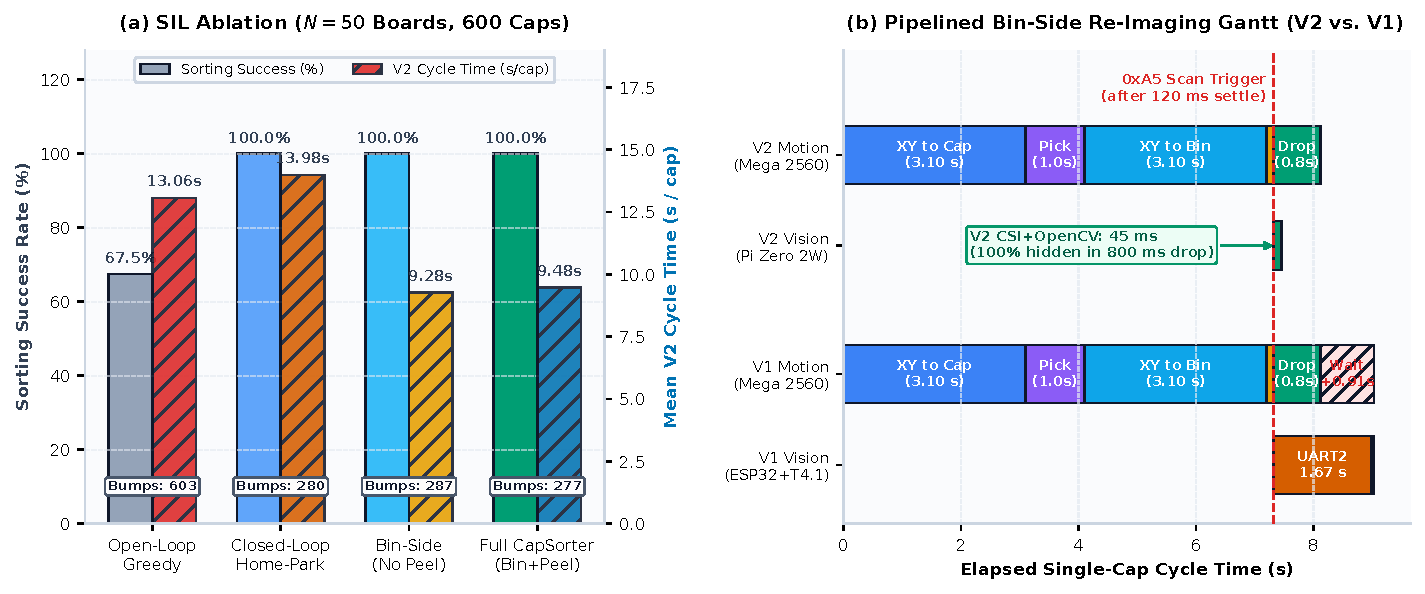
\includegraphics[width=\textwidth]{figures/fig_ablation_and_timing.pdf}
  \caption{Closed-loop policy ablation and pipelined timing analysis. \textbf{(a)}~Monte Carlo SIL comparison ($N=50$ boards, $600$ caps) across four policies: closed-loop re-imaging lifts sorting success from $67.5\%$ to $100.0\%$, while pipelined bin-side scanning reduces V2 cycle time by $32.2\%$ relative to home-park re-imaging and clearance peeling minimizes total neighbor bumps ($277$ vs.\ $603$). \textbf{(b)}~Representative single-cap Gantt timeline showing V2's $45\text{ ms}$ CSI+OpenCV scan completely hidden inside Mega's $800\text{ ms}$ bin drop after \texttt{0xA5}, whereas V1's $1.71\text{ s}$ UART2 stream adds $+0.91\text{ s}$ wait stall.}
  \label{fig:ablation}
\end{figure*}

Three key empirical insights emerge from \cref{tab:ablation}:
\begin{enumerate}
  \item \textbf{Necessity of Closed-Loop Re-Imaging:} Open-loop greedy batching fails on $32.5\%$ of caps ($405/600$ sorted, $603$ physical bumps, $38$ double-sided jaw pinches) because early jaw contacts displace neighboring caps outside capture tolerance. All closed-loop policies achieve \textbf{100.0\% completion} ($600/600$).
  \item \textbf{Pipelined Throughput Advantage:} Returning to $(0,0)$ for every scan (Home-Park Re-Imaging) balloons travel to $855.6\text{ mm/cap}$ and cycle time to $13.98\text{ s/cap}$ (V2). CapSorter's pipelined bin-side re-imaging cuts V2 cycle time by \textbf{32.2\%} ($9.48\text{ s/cap}$, boosting throughput $+47.5\%$ from $4.29$ to $6.33\text{ caps/min}$) and cuts travel by \textbf{40.3\%} ($510.6\text{ mm/cap}$), requiring only $1.70$ clear-FOV verification parks per 12-cap board.
  \item \textbf{Clearance Peeling and Occlusion-Mask Interaction:} Adding X-jaw clearance peeling yields the highest zero-contact clean-pick rate ($54.7\%$) and lowest total neighbor bumps ($277$, a \textbf{54.1\%} reduction vs.\ open-loop) at only a $2.1\%$ cycle-time overhead ($9.48$ vs.\ $9.28\text{ s/cap}$). Notably, Full CapSorter encountered $2$ rare double-pinches ($0.33\%$) versus $0$ in Home-Park: when the $\pm 35\text{ mm}$ bridge-occlusion band transiently masks one outer cap of a tight horizontal triple during a bin-side scan, the adjacent interior cap temporarily appears single-sided. Maintaining short-horizon obstacle persistence across occluded bands is an immediate algorithmic extension.
\end{enumerate}

Finally, \cref{fig:ablation}b and \cref{fig:safety_fsm}b quantify the V1 vs.\ V2 kinematic throughput envelope across all $11{,}664$ board-to-bin transitions ($27\times 27$ grid $\times 4\times 4$ bin pairs). On V2, single-cap cycle time spans $5.00\text{--}12.42\text{ s}$ (mean $8.94\text{ s}$, P95 $12.14\text{ s}$) with $0\text{ ms}$ vision stall because the $45\text{ ms}$ scan finishes well within the $800\text{ ms}$ bin drop. On V1, the $1.67\text{ s}$ UART2 stream plus $\sim 40\text{ ms}$ C++ processing exceeds the $800\text{ ms}$ drop by $+0.91\text{ s/cap}$, shifting the cycle distribution to $5.91\text{--}13.33\text{ s}$ (mean $9.85\text{ s}$, P95 $13.05\text{ s}$).

\begin{figure*}[t]
  \centering
  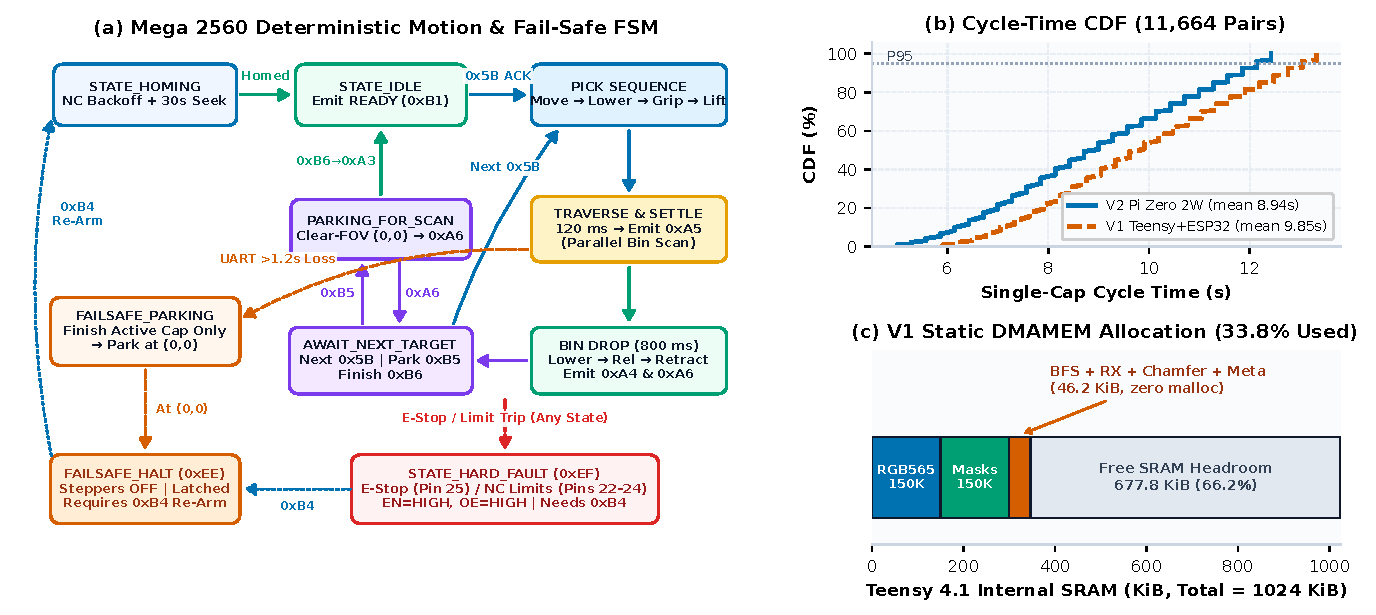
\includegraphics[width=\textwidth]{figures/fig_safety_fsm_and_memory.pdf}
  \caption{Real-time safety architecture, kinematic throughput envelope, and bare-metal memory footprint. \textbf{(a)}~Deterministic Mega~2560 FSM governing normal closed-loop pick-place cycles, bin-side \texttt{0xA5} scanning, clear-FOV verification parking (\texttt{0xB5}), comms-loss finish-active-cycle-and-park recovery (\texttt{0xEE}), and hard-fault E-stop/limit latching (\texttt{0xEF}) requiring explicit \texttt{0xB4} re-arming. \textbf{(b)}~Analytical cumulative distribution of single-cap cycle time across $11{,}664$ workspace-to-bin pairs showing V2's $0.91\text{ s/cap}$ pipelined latency-hiding advantage over V1. \textbf{(c)}~Teensy~4.1 static \texttt{DMAMEM} utilization ($375.0\text{ KiB} / 1024\text{ KiB} = 36.6\%$ with $8{,}192$-entry BFS queue, zero heap allocation).}
  \label{fig:safety_fsm}
\end{figure*}

% =========================================================================
% SECTION 6: LIMITATIONS, BENCH GATE & FUTURE WORK
% =========================================================================
\section{Limitations, Bench Validation Gate, and Future Work}
\label{sec:limitations}

In strict adherence to engineering transparency, CapSorter is currently at the \textbf{pre-validation firmware and SIL verification stage}; physical bench validation on assembled hardware is mandatory prior to production deployment:
\begin{enumerate}
  \item \textbf{Electro-Mechanical SKU and Thermal Sign-Off:} Exact TMC2208 carrier sense resistors ($R_{\mathrm{sense}}$) must be measured before tuning $V_{\mathrm{ref}}$ via \cref{eq:tmc_irms}. Servo SKU voltage limits (e.g., $4.8\text{ V}$ nominal for TowerPro MG90S), PCA9685 \texttt{V+} rail droop under simultaneous stall, V2 Branch~C \texttt{PWR IN} $5\text{ V}$ rail stability under combined Pi + $3.5\text{ in}$ LCD + IMX219 + CH9102 load (confirming CH9102 \texttt{+5V} remains open), UART logic waveforms at receiving pins, and Z-axis counterbalance spring behavior under E-stop power removal must be verified experimentally.
  \item \textbf{Polled Limit-Switch Stopping Distance and Physical Calibration:} Because Mega Pins~22--24 are polled on ATmega2560 Port~A, actual mechanical overrun distance at $70\text{ mm/s}$ must be measured on the bench alongside physical \texttt{STEPS\_PER\_MM}, \texttt{TOOL\_OFFSET\_X/Y}, and real checkerboard captures covering all four frame corners under the installed diffused LED light plate.
  \item \textbf{Specular Glare and Grip Verification:} Glossy or translucent caps under oblique ambient light can fragment HSV masks; deploying the optional physical cap-presence microswitch (\texttt{HAS\_GRIP\_SENSOR=1} on Pin~26) will upgrade open-loop grip confirmation to closed-loop grasp verification.
  \item \textbf{Staged Hardware Bring-Up Protocol (Stages~0--8):} To prevent commissioning damage from deploying full autonomous firmware onto unverified hardware, the repository provides a dedicated step-by-step manual (\texttt{firmware/HARDWARE\_BRINGUP\_GUIDE.md}) and 8 isolated bench tools (\texttt{firmware/bringup/}): three Mega~2560 sketches (zero-motion NC switch/E-stop verifier, interactive PCA9685 servo tick calibrator, and slow stepper polarity/homing/\texttt{STEPS\_PER\_MM}/\texttt{TOOL\_OFFSET}/bin finder) plus five Pi Zero~2~W tools (live cap bounding-box/HSV preview over MJPEG browser stream or LCD, checkerboard capture and 4-corner pixel ruler/calibration generator, calibrated millimeter/clearance verifier, binary UART ping/single-pick/cut tester, and 3.5\,in SPI LCD touch-axis calibrator).
\end{enumerate}

Promising algorithmic extensions include: (i)~\emph{occlusion-aware obstacle memory} persisting previously observed caps inside the $\pm 35\text{ mm}$ bridge band during bin-side scans to eliminate the $0.33\%$ residual double-pinch rate; (ii)~deploying a quantized MobileNet/YOLO-nano classifier on V2's quad-core Cortex-A53 to classify deformed, transparent, or multi-colored branded caps beyond HSV thresholds; and (iii)~closed-loop stepper encoder feedback for absolute slip detection.

% =========================================================================
% SECTION 7: CONCLUSION
% =========================================================================
\section{Conclusion}
\label{sec:conclusion}

We presented \textbf{CapSorter}, an air-gapped, dual-controller vision-guided Cartesian bottle-cap sorting architecture spanning both a bare-metal microcontroller stack (V1: ESP32-CAM + Teensy~4.1) and a consolidated offline Linux edge stack (V2: Sony IMX219 $160^\circ$ CSI + Raspberry Pi Zero~2~W + $3.5\text{ in}$ SPI Touch LCD HUD bridged via Micro-USB OTG CH9102/CP2102), united over a shared CRC-16/CCITT-FALSE binary protocol with a deterministic Arduino Mega~2560 motion and safety layer. Through fail-closed lens calibration, closed-form radial cap-height parallax compensation, distance-transform splitting of touching same-color caps, X-jaw clearance-first peeling, and pipelined bin-side re-imaging, CapSorter eliminates open-plate bump failures ($100.0\%$ vs.\ $67.5\%$ sorting completion) while hiding V2's entire $45\text{ ms}$ perception pipeline inside the $800\text{ ms}$ bin-drop sequence ($9.48\text{ s/cap}$, $32.2\%$ faster than home-park re-imaging). While V1 proves that complete closed-loop vision sorting fits deterministically within $375.0\text{ KiB}$ of microcontroller SRAM, V2 delivers markedly superior cluster-splitting recall ($100.0\%$ vs.\ $82.4\%$ on dense $3\times 3$ clusters), sub-millimeter wide-angle accuracy ($0.29\text{ mm}$ mean), zero vision stall overhead, and standalone local operator monitoring/re-arming—establishing a rigorous, reproducible, and safety-first blueprint for accessible offline robotic sorting.

{
  \small
  \bibliographystyle{ieeenat_fullname}
  \bibliography{references}
}

% =========================================================================
% APPENDIX (Fresh Page After References per Conference Formatting Standards)
% =========================================================================
\clearpage
\appendix
\onecolumn

\section{Complete Hardware Pinout and Interface Matrix}
\label{app:pinout}

To support full hardware reproducibility across both V1 and V2 configurations, \cref{tab:pinout} consolidates every electrical signal, controller pin assignment, operating logic level, and safety constraint enforced in the firmware vault (\texttt{firmware/mega\_motion/mega\_motion.ino}, \texttt{v1\_teensy41/teensy\_vision.cpp}, \texttt{v1\_esp32cam/esp32cam\_uart.ino}, \texttt{v2\_pizero2w/pi\_zero\_vision.py}, and \texttt{v2\_pizero2w/lcd\_hud.py}).

\begin{table}[h]
  \centering
  \small
  \resizebox{\textwidth}{!}{%
  \begin{tabular}{@{}lllll@{}}
    \toprule
    \textbf{Subsystem Interface} & \textbf{Source Board / Pin} & \textbf{Destination Board / Pin} & \textbf{Bus / Logic Level} & \textbf{Critical Safety / Timing Rule} \\
    \midrule
    \multicolumn{5}{@{}l}{\textit{Version 1 Vision Front-End (Bare-Metal Dual-MCU)}} \\
    ESP32-CAM $\to$ Teensy Frame Link & ESP32 GPIO13 (TX2) / GPIO14 (RX2) & Teensy Pin~7 (RX2) / Pin~8 (TX2) & UART2 @ $921.6\text{ kbps}$ ($3.3\text{ V}$) & $16\text{ KiB}$ DMA RX buffer; PSRAM required \\
    Teensy $\leftrightarrow$ Mega Command Link & Teensy Pin~1 (TX1) / Pin~0 (RX1) & Shifter LV $\leftrightarrow$ HV $\leftrightarrow$ Mega Pin~19/18 & UART1 @ $115.2\text{ kbps}$ ($3.3\leftrightarrow 5\text{ V}$) & Mandatory bidirectional shifter on TX \& RX \\
    \midrule
    \multicolumn{5}{@{}l}{\textit{Version 2 Vision \& HMI Front-End (Consolidated Edge SBC)}} \\
    IMX219 $160^\circ$ Camera $\to$ Pi Zero~2~W & 8MP IMX219 22-Pin CSI Ribbon & Pi Zero~2~W MIPI CSI-2 Port & 2-Lane MIPI CSI-2 ($\sim 20\text{ ms}$) & Full-sensor $1640{\times}1232$ $2{\times}2$ binning \\
    Pi Zero~2~W $\leftrightarrow$ $3.5\text{ in}$ SPI Touch LCD & GPIO Pins~1--26 (SPI0 + GPIO~17/24/25) & LCD V3.0 26-Pin Female Header & $3.3\text{ V}$ SPI0 / $5\text{ V}$ BL (\texttt{/dev/fb0}) & \texttt{piscreen,drm}; power Pi via \texttt{PWR IN} \\
    Pi Zero~2~W $\leftrightarrow$ Mega Command Link & Inner Micro-USB OTG $\to$ CH9102/CP2102 & Shifter LV (\texttt{3V3}) $\leftrightarrow$ HV $\leftrightarrow$ Mega~19/18 & USB-TTL @ $115.2\text{ kbps}$ ($3.3\leftrightarrow 5\text{ V}$) & \texttt{/dev/capsorter\_mega}; leave \texttt{+5V} open! \\
    \midrule
    \multicolumn{5}{@{}l}{\textit{Shared Deterministic Motion, Servo, and Safety Layer (Arduino Mega~2560)}} \\
    X-Axis TMC2208 Driver & Mega Pin~2 (STEP), Pin~5 (DIR) & TMC2208\_X STEP / DIR & $5.0\text{ V}$ Digital ($40\text{ steps/mm}$) & \texttt{MS1=MS2=GND} ($1/8$ StealthChop2) \\
    Y-Axis TMC2208 Driver & Mega Pin~3 (STEP), Pin~6 (DIR) & TMC2208\_Y STEP / DIR & $5.0\text{ V}$ Digital ($40\text{ steps/mm}$) & \texttt{MS1=MS2=GND}; $100\,\mu\text{F}$ on \texttt{VMOT} \\
    Shared Stepper Hardware Enable & Mega Pin~8 (\texttt{PIN\_STEPPER\_EN}) & Both TMC2208 \texttt{EN} pins & Active-LOW ($5.0\text{ V}$) & Driven \texttt{HIGH} at boot, halt, and fault \\
    PCA9685 Servo Controller & Mega Pin~20 (SDA), Pin~21 (SCL), Pin~9 (OE) & PCA9685 (\texttt{0x40}) SDA / SCL / OE & $400\text{ kHz}$ I2C ($5.0\text{ V}$) & CH0 = Z-Lift, CH1 = X-Jaw; \texttt{OE=HIGH} on fault \\
    Polled NC Limit Switches (X, Y, Z) & Mega Pins~22 (X), 23 (Y), 24 (Z) & NC Microswitches to Common GND & \texttt{INPUT\_PULLUP} ($5.0\text{ V}$) & Port~A (no ISR); $8\text{ ms}$ timed debounce; step-bounded home \\
    Dual-Pole Latching E-Stop & Pole~1: $12\text{ V}$ $\to$ Branches A \& B; Pole~2: Pin~25 & Actuator Power Cut + Mega \texttt{PIN\_ESTOP} & Hardwired $12\text{ V}$ + NC Sense & Branch~C bypasses E-stop; $4\text{ ms}$ debounce latches \texttt{0xEF} \\
    Optional Grip-Presence Sensor & Mega Pin~26 (\texttt{PIN\_GRIP\_SENSE}) & Gripper Microswitch to GND & Active-LOW (\texttt{HAS\_GRIP\_SENSOR}) & Disabled (\texttt{0}) by default until fitted \\
    \bottomrule
  \end{tabular}}
  \caption{Complete pin-by-pin electrical interface and safety wiring matrix across CapSorter V1, V2, and shared Mega~2560 hardware.}
  \label{tab:pinout}
\end{table}

\section{Categorized Bill of Materials (V1 and V2)}
\label{app:bom}

\Cref{tab:bom} summarizes the mechanical, actuation, vision, and power components across both architectures, noting SKU verification items required during physical bench integration (\cref{sec:limitations}).

\begin{table}[h]
  \centering
  \small
  \resizebox{\textwidth}{!}{%
  \begin{tabular}{@{}clcll@{}}
    \toprule
    \textbf{\#} & \textbf{Component} & \textbf{Qty} & \textbf{Engineering Specification} & \textbf{Architectural Role \& Scope} \\
    \midrule
    01a & Teensy~4.1 \emph{(V1 only)} & 1 & ARM Cortex-M7 @ $600\text{ MHz}$, $1024\text{ KiB}$ SRAM & V1 vision decoding, chamfer split, 4-pt DLT \\
    01b & ESP32-CAM AI-Thinker \emph{(V1 only)} & 1 & Xtensa LX6 @ $240\text{ MHz}$ + OV2640 + PSRAM & V1 top-down QVGA RGB565 UART2 streamer \\
    02a & Raspberry Pi Zero~2~W + 16\,GB SD \emph{(V2 only)} & 1 & $4\times$ Cortex-A53 @ $1.0\text{ GHz}$, $512\text{ MB}$ RAM & V2 consolidated offline OpenCV vision \& native HUD \\
    02b & 8MP Sony IMX219 $160^\circ$ Camera \emph{(V2 only)} & 1 & $160^\circ$ wide-angle CSI + 22-pin ribbon & V2 $640{\times}480$ RGB888 top-down acquisition \\
    02c & $3.5\text{ in}$ SPI Touch LCD V3.0 \emph{(V2 only)} & 1 & $480{\times}320$ HVGA TFT, ILI9486 + XPT2046 (26-pin) & V2 local animated cap/gantry HUD \& touch Re-Arm \\
    02d & Official OTG Adapter + CH9102/CP2102 \emph{(V2 only)} & $1+1$ & Micro-USB OTG cable + 5-pin USB-TTL UART bridge & V2 \texttt{/dev/capsorter\_mega} link while GPIO drives LCD \\
    03 & Arduino Mega~2560 Rev3 & 1 & ATmega2560 @ $16\text{ MHz}$, $54$ I/O, 4 UARTs & Shared deterministic motion FSM \& safety watchdog \\
    04 & PCA9685 16-Ch PWM Driver & 1 & NXP PCA9685, 12-bit $50\text{ Hz}$ I2C (\texttt{0x40}) & Jitter-free Z-lift and parallel gripper PWM \\
    05 & MG90S Metal-Gear Micro Servos & 2 & $\sim 2.2\text{ kg}\cdot\text{cm}$ torque (verify $4.8\text{ V}$ SKU) & Z-axis crank-slider stroke ($40\text{ mm}$) \& X-jaws \\
    06 & NEMA~17 Stepper Motors & 2 & $40\text{ mm}$ body, $1.3\text{ A/phase}$, $4.2\text{ kg}\cdot\text{cm}$ & X and Y moving-bridge Cartesian belt drives \\
    07 & TMC2208 V1.2 SilentStepStick Drivers & 2 & StealthChop2, $1/8$ microstep, heatsink (verify $R_{\mathrm{sense}}$) & Quiet XY step actuation (\cref{eq:tmc_irms}) \\
    08 & GT2 Timing Belts \& 20T Pulleys & 2 sets & $6\text{ mm}$ width, $2\text{ mm}$ pitch, $5\text{ mm}$ bore pulleys & $40.0\text{ mm/rev}$ linear gantry transmission \\
    09 & 2020 V-Slot Extrusions \& V-Wheel Kits & 1 set & Anodized aluminum profiles + Delrin carriages & Rigid $500{\times}500{\times}500\text{ mm}$ frame + plywood plate \\
    10 & $12\text{ V}/10\text{ A}$ Industrial SMPS & 1 & $120\text{ W}$ master DC supply & Common star-ground primary supply (Branches A--C) \\
    11 & $5\text{ V}/5\text{ A}$ Servo Buck + $1{,}000\,\mu\text{F}$ Cap & 1 & Step-down $12\text{ V}\to 5\text{ V}$ (switched via E-stop Pole~1) & Dedicated regulated Branch~B servo rail (\texttt{PCA9685 V+}) \\
    12 & $5\text{ V}/3\text{ A}$ Logic Buck Converter & 1 & Step-down $12\text{ V}\to 5\text{ V}$ (bypasses E-stop) & Always-on Branch~C rail (Mega \texttt{5V} + V2 Pi \texttt{PWR IN}) \\
    13 & 4-Ch Bidirectional Level Shifter & 1 & $3.3\text{ V}\leftrightarrow 5.0\text{ V}$ MOSFET translator & Shifts V1 Teensy / V2 CH9102-CP2102 (\texttt{LV}$\leftarrow$\texttt{3V3}, \texttt{+5V} open) \\
    14 & NC Limit Switches + Dual-Pole E-Stop & $3+1$ & Roller-lever NC microswitches + $\ge 10\text{ A}$ latching mushroom & Polled X/Y/Z limits + hardwired actuator cutoff \\
    15 & Diffused White LED Light Plate & 1 & Uniform overhead shadow-free backlight/panel & Stabilizes HSV color segmentation under fixed AWB \\
    \bottomrule
  \end{tabular}}
  \caption{Categorized Bill of Materials (BOM) for CapSorter V1 and V2 hardware builds.}
  \label{tab:bom}
\end{table}

\end{document}
